\section{EVALUATION}
\uline{\textbf{Simulations}}: 
The proposed algorithm for platonic solids path planning by rolling through edge contact was implemented in MATLAB environment. 
In general of path planning, there are three case studies including same location and different orientation between initial configuration and goal configuration, long distance between two configurations, and bi-direction path finding. To validate the proposed algorithm, this study only considers the first case study of path planning that both initial and goal configuration have the same positions and different orientations.\\  

\noindent\uline{\textbf{Cube solid}}:
The cube has a length which is the same as the length of side of each grid square. The only way to move from initial position to goal position is by rolling from square to square without moving diagonal. The Figure \ref{fig:cubePath0} shows the first three layers of cube path finding on the grid. The algorithm implements in $O(|E|^3)$ running time from the second layer. The executed time can be reduced when the updated cubes achieved the same configurations. The $*$ position in the grid is occupied by the two updated cubes with different orientations. To be more visualized, the Figure \ref{fig:Cube1Case1} indicates the first step of rolling of the cube with its coordinates in three arrows red, green and blue colors. Four paths of cube rolling are shown in the Figure \ref{fig:Cube2Case1}.

\begin{figure}[h]
\centering
	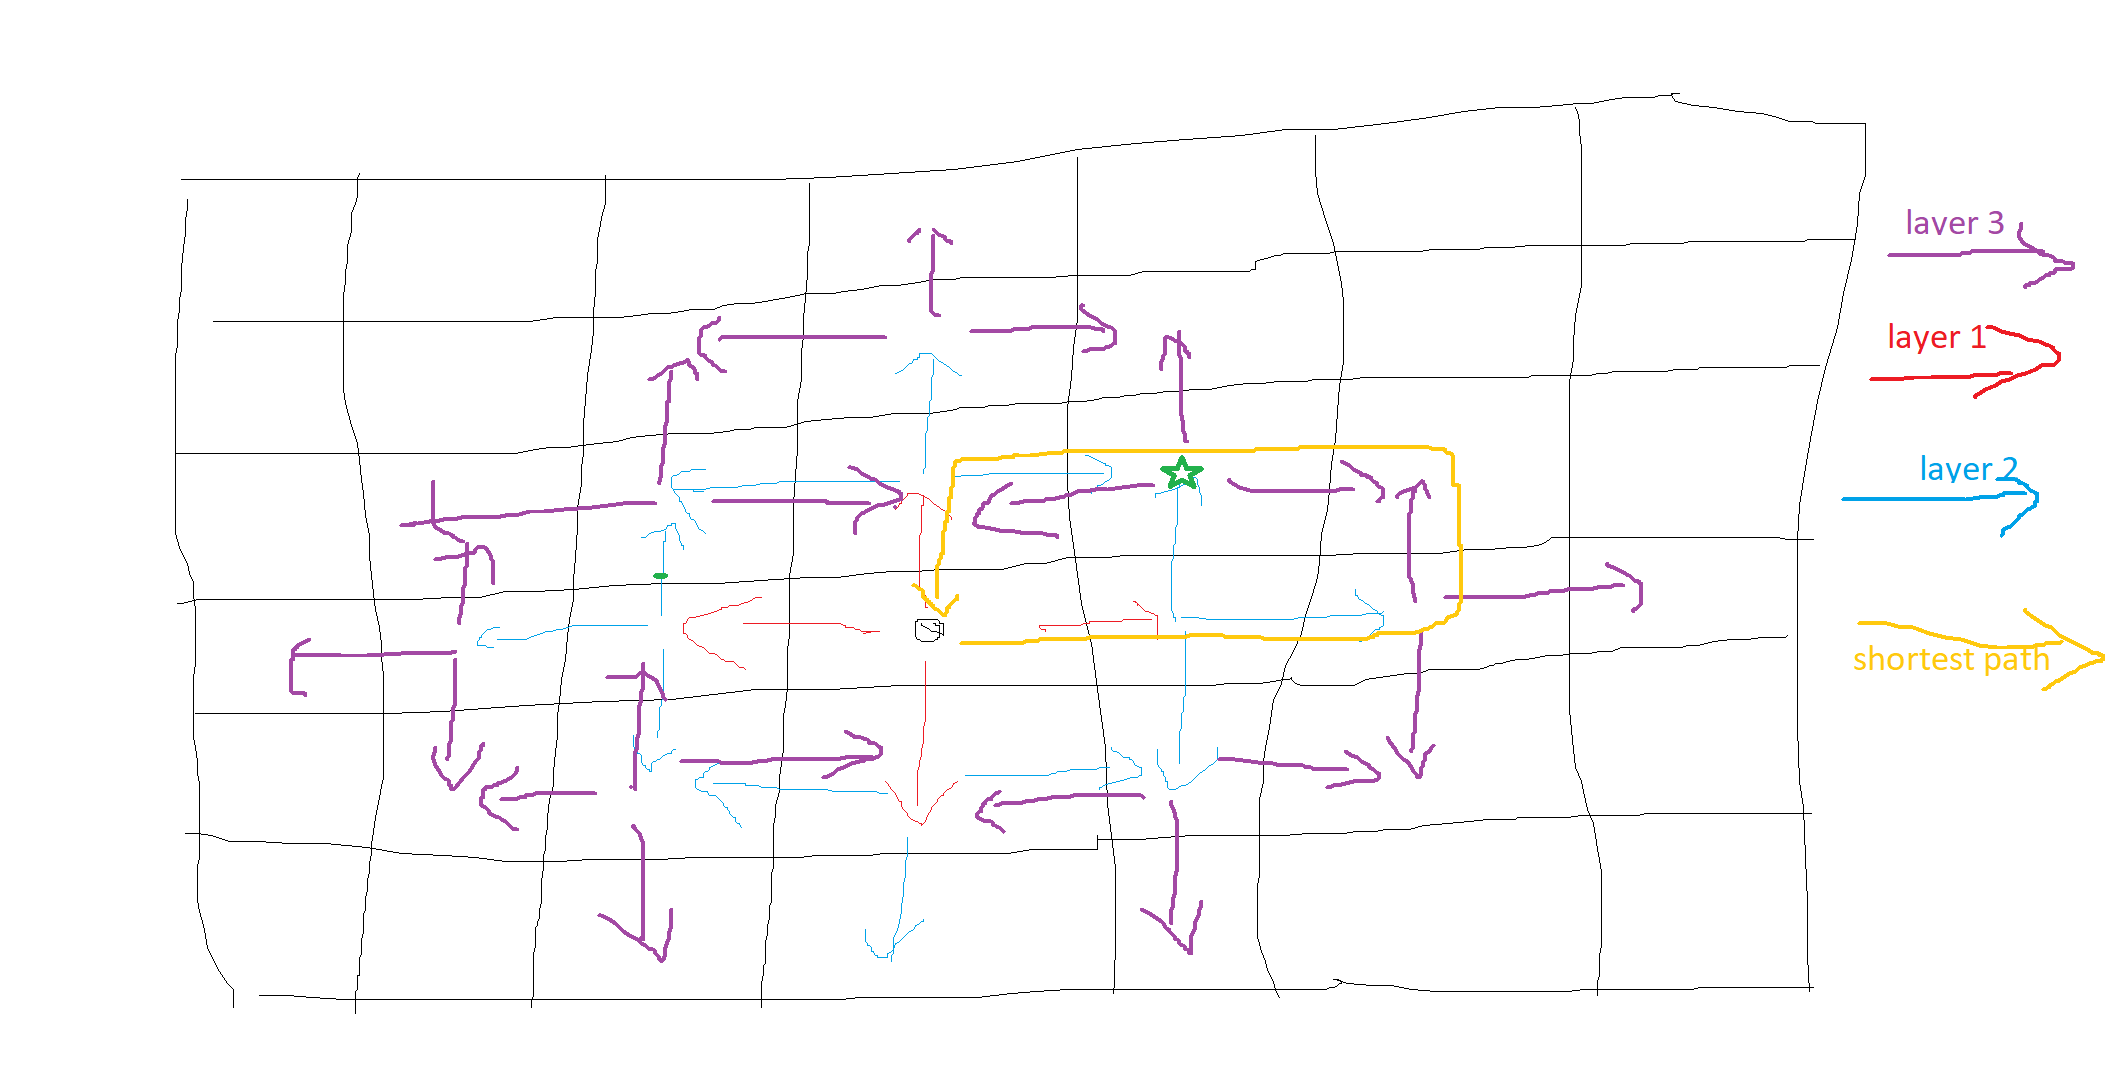
\includegraphics[width=1\textwidth]{image/cubePath0.png}
	\caption{The first three layers of cube rolling}
	\label{fig:cubePath0}
\end{figure}



\noindent ABC here.

\begin{center}
\begin{figure}[h]
\subfigure[The initial configuration is the same position but different orientation with goal configuration]{
	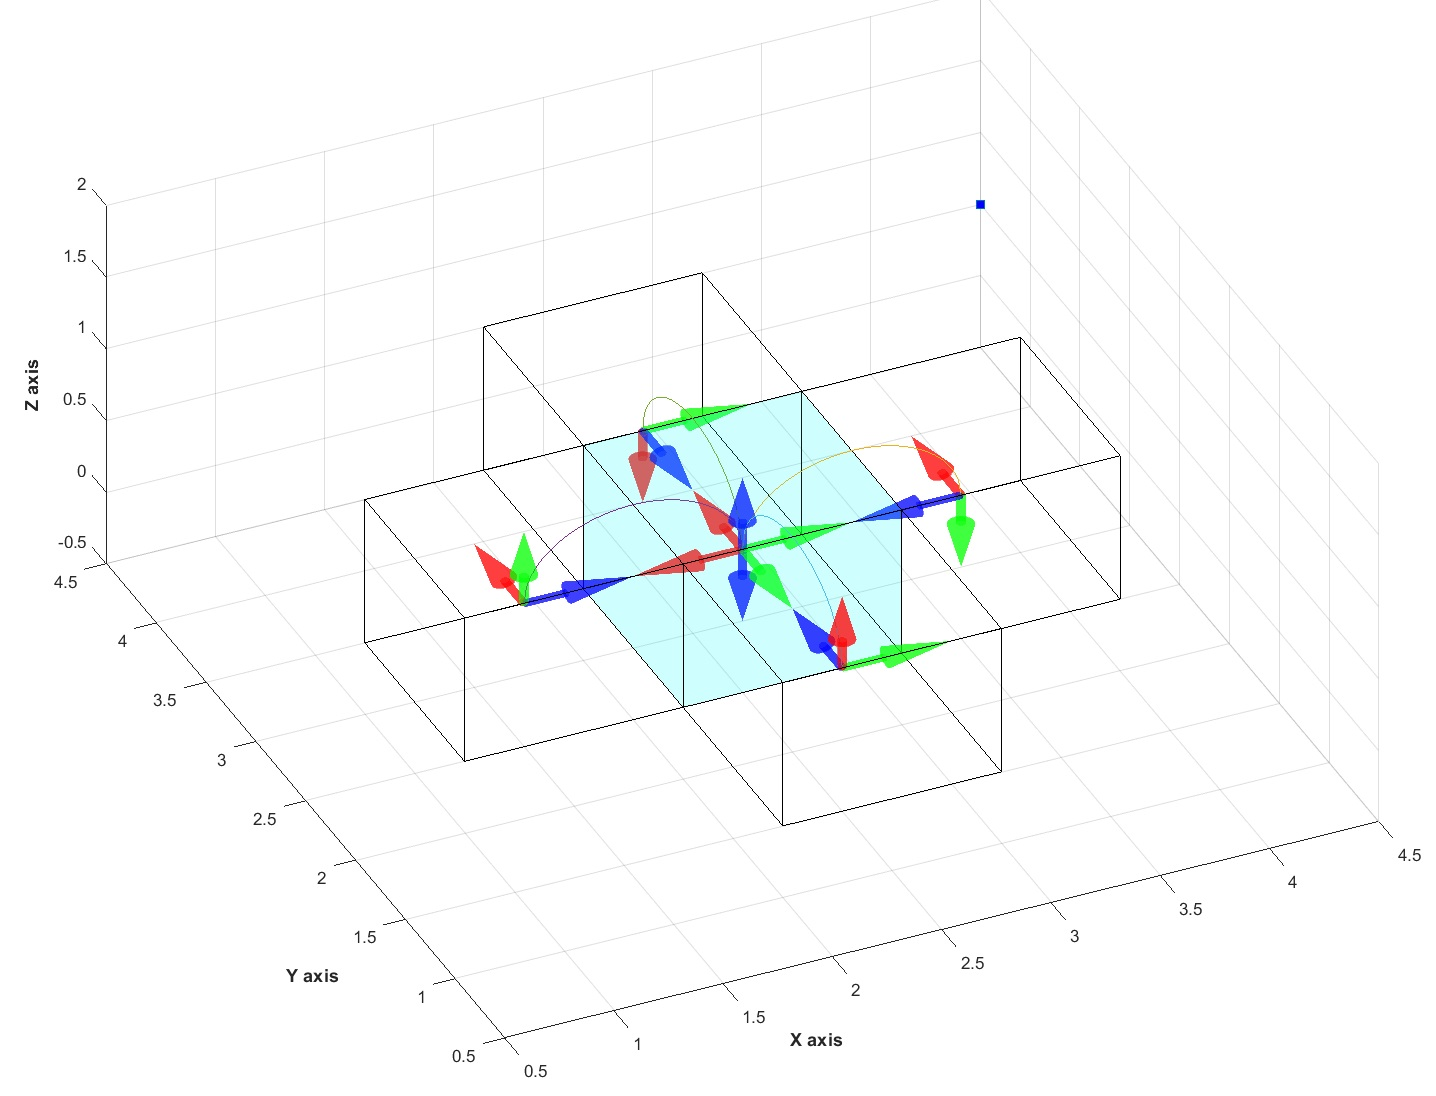
\includegraphics[width=0.5\textwidth]{image/cube11.jpg}
	\label{fig:Cube1Case1}
	}
\hfill
\subfigure[First four paths of the cube rolling]{
	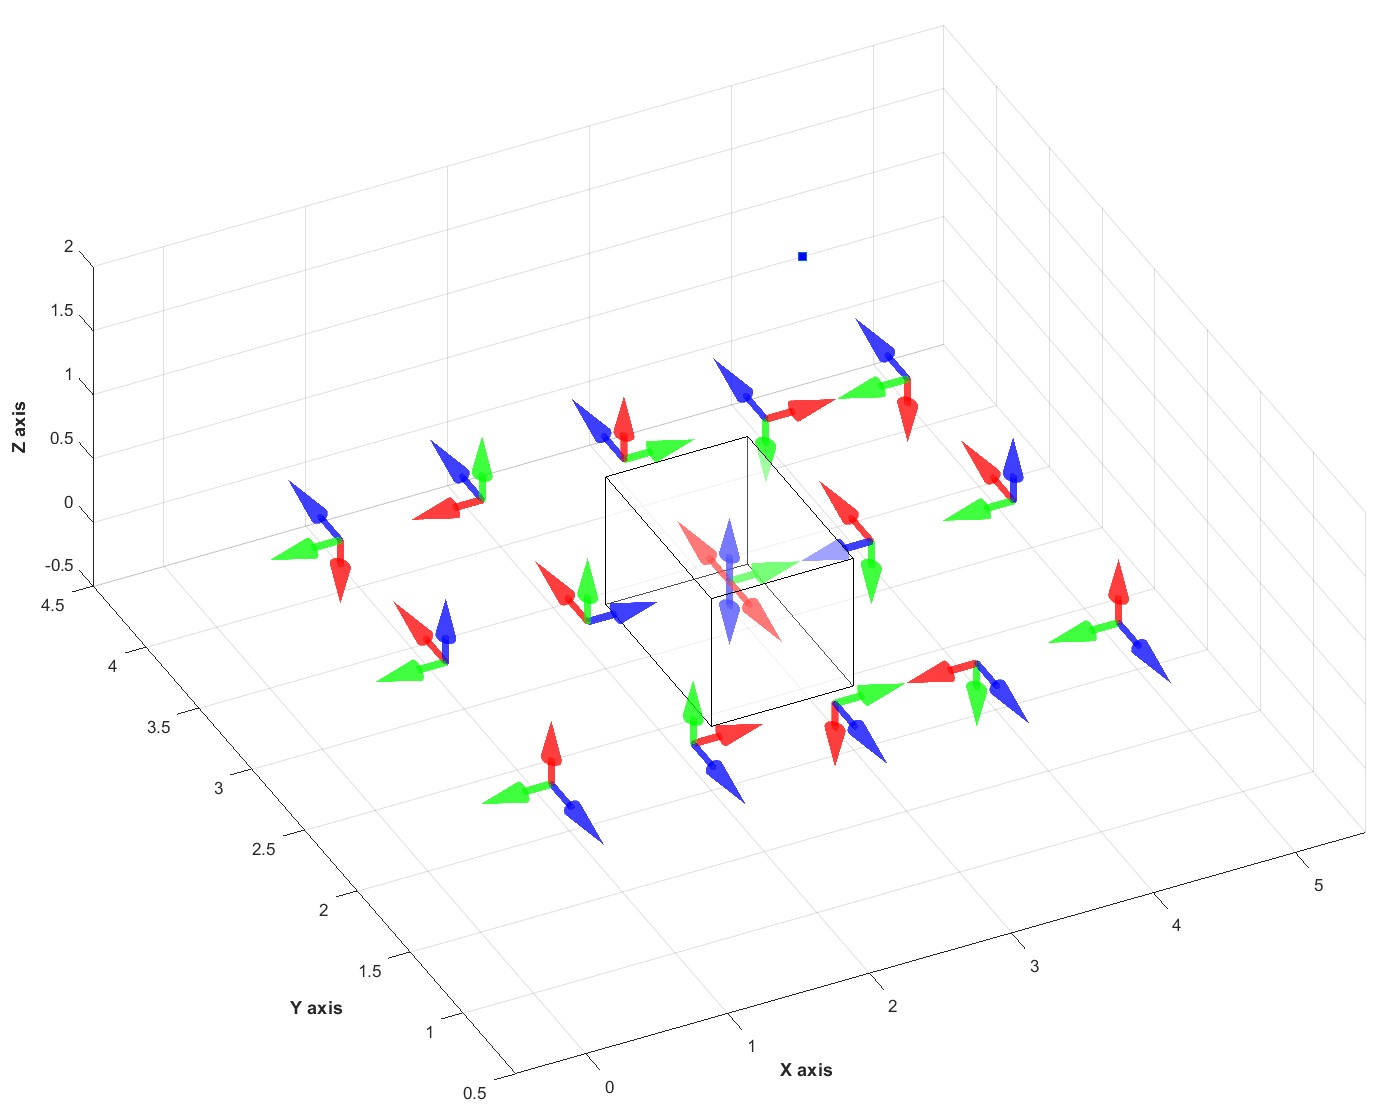
\includegraphics[width=0.5\textwidth]{image/cubePath4Dirs.jpg}
%    \includegraphics[page=2,width=.5\textwidth]{image/test2.pdf}	
	\label{fig:Cube2Case1}
	}
\caption{Blah Blah}
\end{figure}
\end{center}

\noindent\uline{Result}: 
\begin{figure}[h]
\centering
	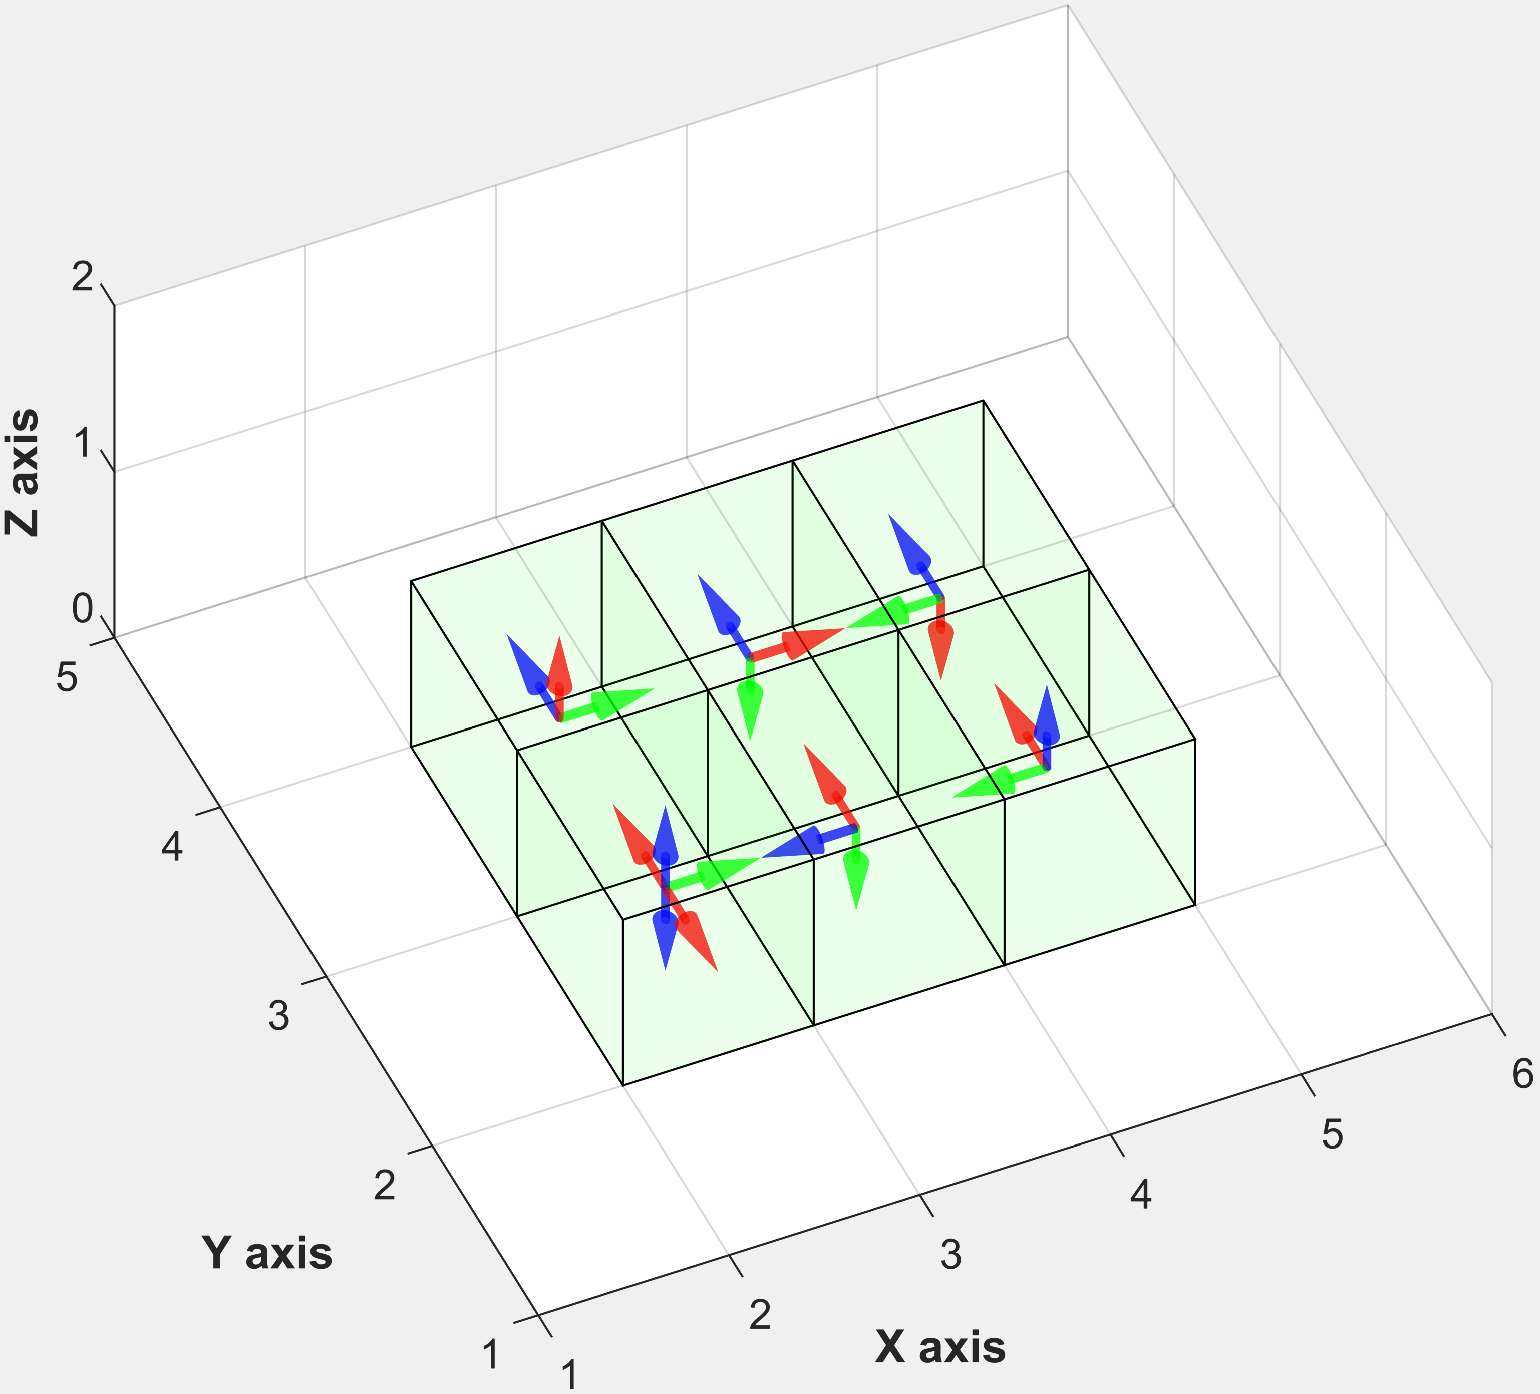
\includegraphics[width=0.5\textwidth]{image/cubePath1.pdf}
%	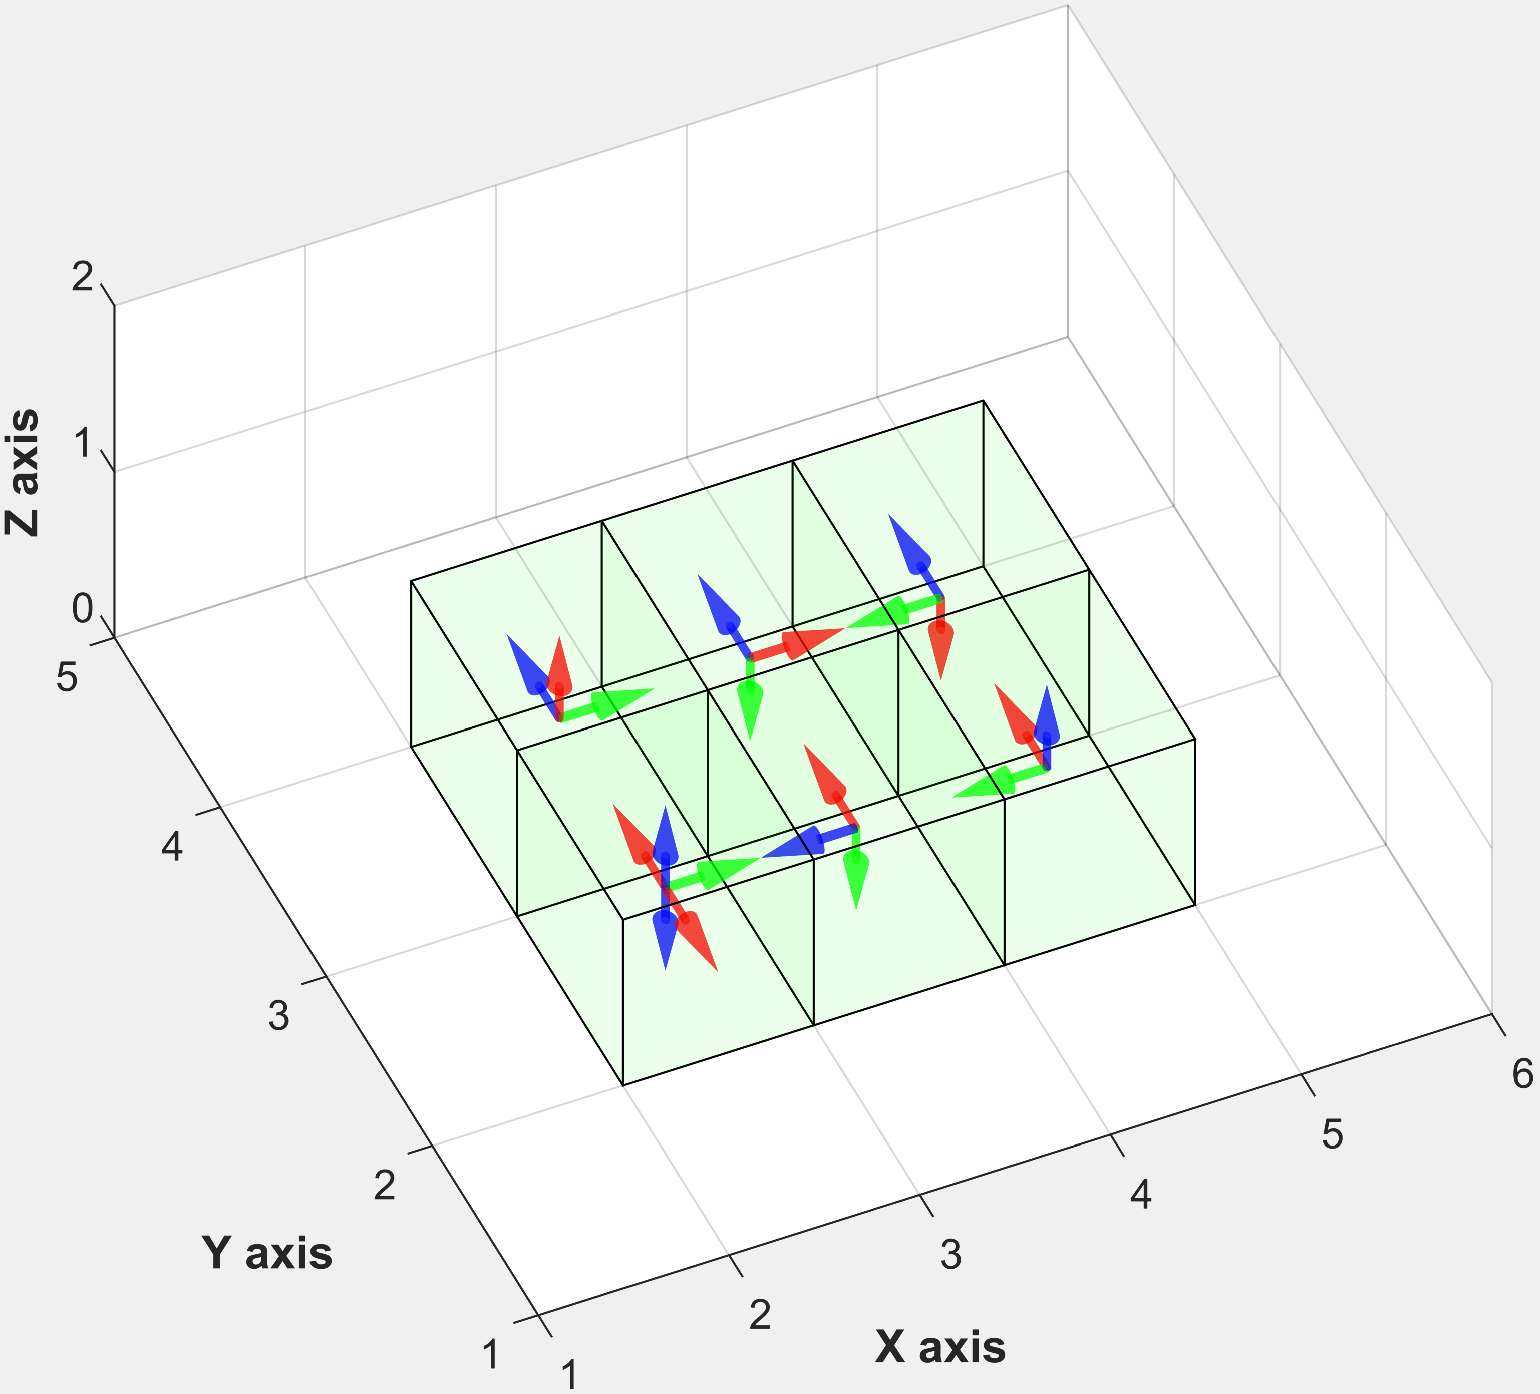
\includepdf[pages=-,pagecommand={},width=0.5\textwidth]{image/cubePath1.pdf}
	\caption{Shortest path of cube rolling}
	\label{fig:cubePath1}
\end{figure}



%\begin{figure}[h]
%	\centering
%		\begin{subfigure}[t]
%			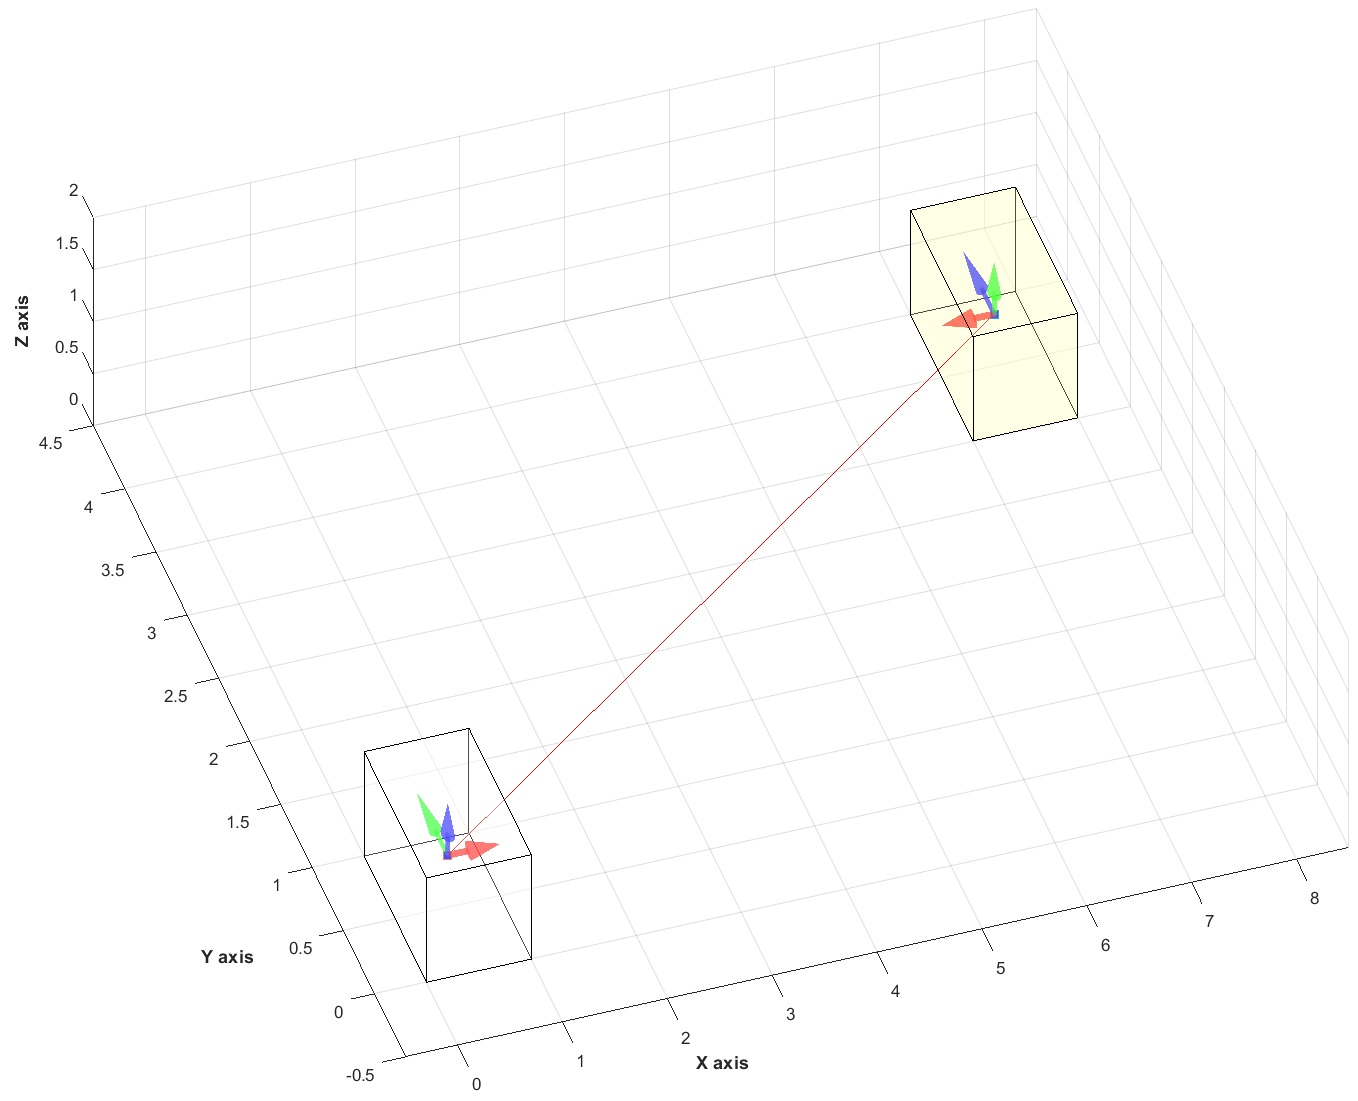
\includegraphics[width=0.5\textwidth]{image/cubePathCase2Initial.jpg}
%			\subcaption{Long distance between two configurations}
%			\label{fig:Cube1Case2}
%		\end{subfigure}
%%\hfill
%		\begin{subfigure}[t]
%			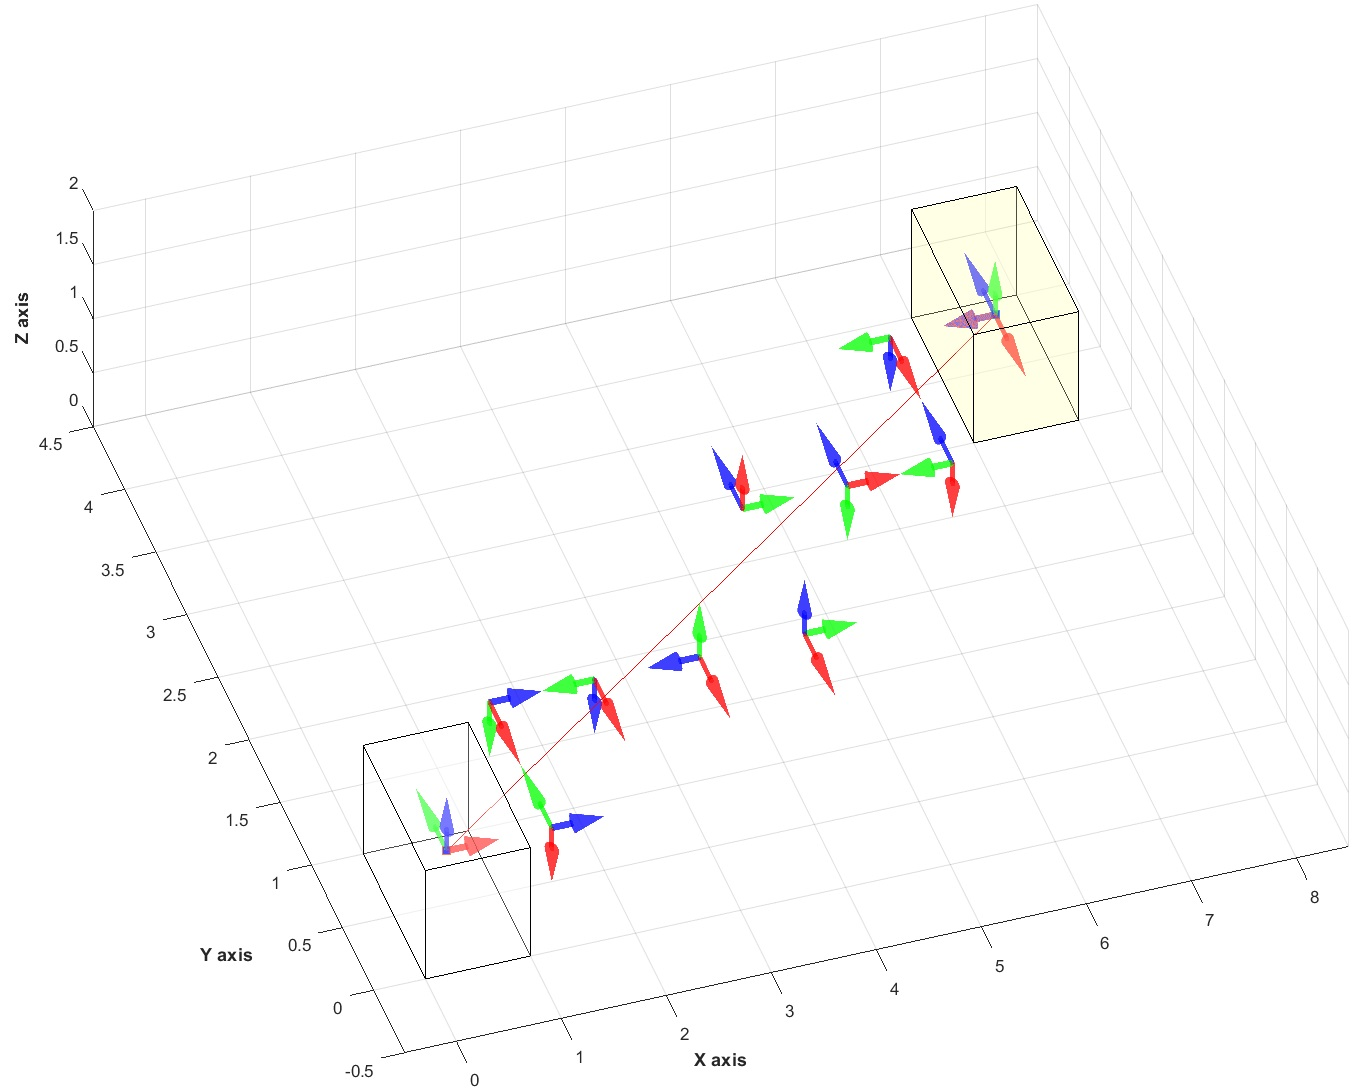
\includegraphics[width=0.5\textwidth]{image/cubePathCase2DirecRolling.jpg}
%			\subcaption{Directly rolling from initial configuration to goal configuration}
%			\label{fig:Cube2Case2}
%		\end{subfigure}
%\end{figure}

%%
%%
%%
\clearpage
\newpage
\noindent Although considering the case study within 
The proposed algorithm in this study can be applied for the case study of long distance between the initial and goal configurations. 
Figure \ref{fig:cubeLongDist} shows an example with two different paths.
Shortest path-finding algorithm is added to the original algorithm to find the shortest path from start point to the goal point. 
After finishing this step, the cube updated to a new orientation with different orientation at the goal configuration. Then, the original algorithm will be implemented from the updated cube to the goal configuration.
Assume that the initial configuration is at $S_1$ and the goal configuration is at $S2$. In the first step, the red segment $S_1S_2$ shows the shortest distance from start position to goal position. The cube will roll through this segment and achieve the updated orientation at the goal position called shortest path for the case of long distance. 

\begin{center}
\begin{figure}[h]
\subfigure[Path1]{
	\includegraphics[width=0.5\textwidth]{image/cubeCase2Path1.jpg}
	\label{fig:cubeLongDistPath1}
	}
\hfill
\subfigure[Path2]{
	\includegraphics[width=0.5\textwidth]{image/cubeCase2Path2.jpg}
	\label{fig:cubeLongDistPath2}
	}
\caption{The case study of long distance between the initial and goal configurations}
\label{fig:cubeLongDist}
\end{figure}
\end{center}
%%
%%
%%
%%
%%==================================================================================
%%
%%==================================================================================
%%
%%
%%
\clearpage
\newpage
\noindent\uline{\textbf{Tetrahedron solid}}:
Writing about cube solid properties\\

\noindent\uline{Case study 1}:
Dennis also went his own way and divided the sides of the triangles into equal-angles (as measured from the center of the geodesic), instead of equal-length pieces. This technique is slightly more effective at evenly distributing the triangles across the surface of the sphere. For example, compare an octahedron subdivided with frequency 20, using the linear technique (as outlined by the quiz) versus the angular technique Dennis used in this picture. Note how the linear technique has the triangles piling up along the edges of the original face of the octahedron, where the radial technique does a better job of spacing them out.\\

\begin{center}
\begin{figure}[h]
\subfigure[The initial configuration is the same position but different orientation with goal configuration]{
	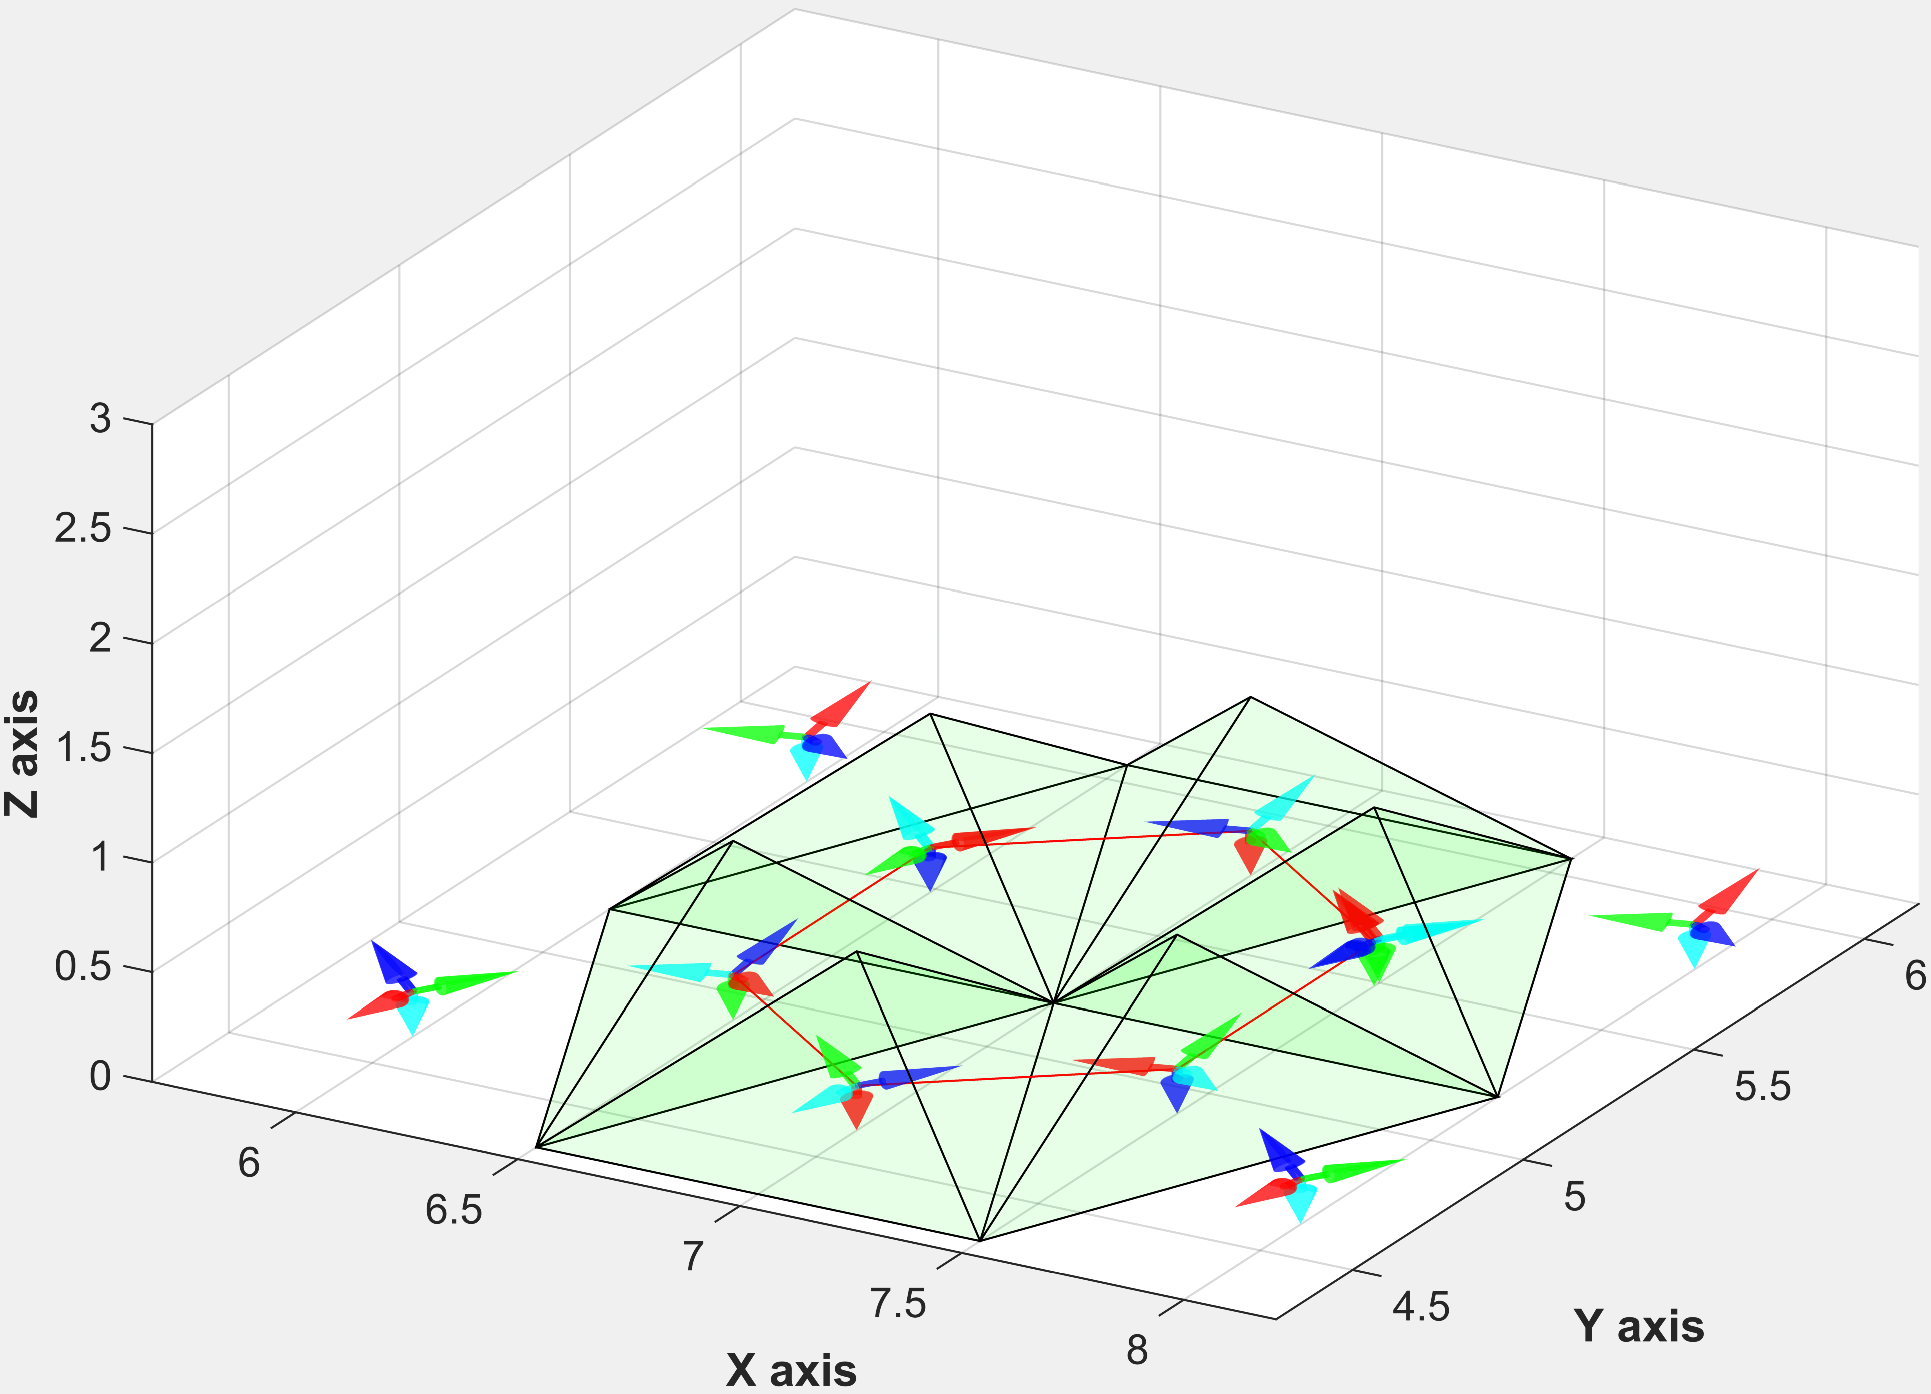
\includegraphics[width=0.5\textwidth]{image/tetraPath2.pdf}
	\label{fig:Tetra1Case1}
	}
\hfill
\subfigure[First four paths of the cube rolling]{
	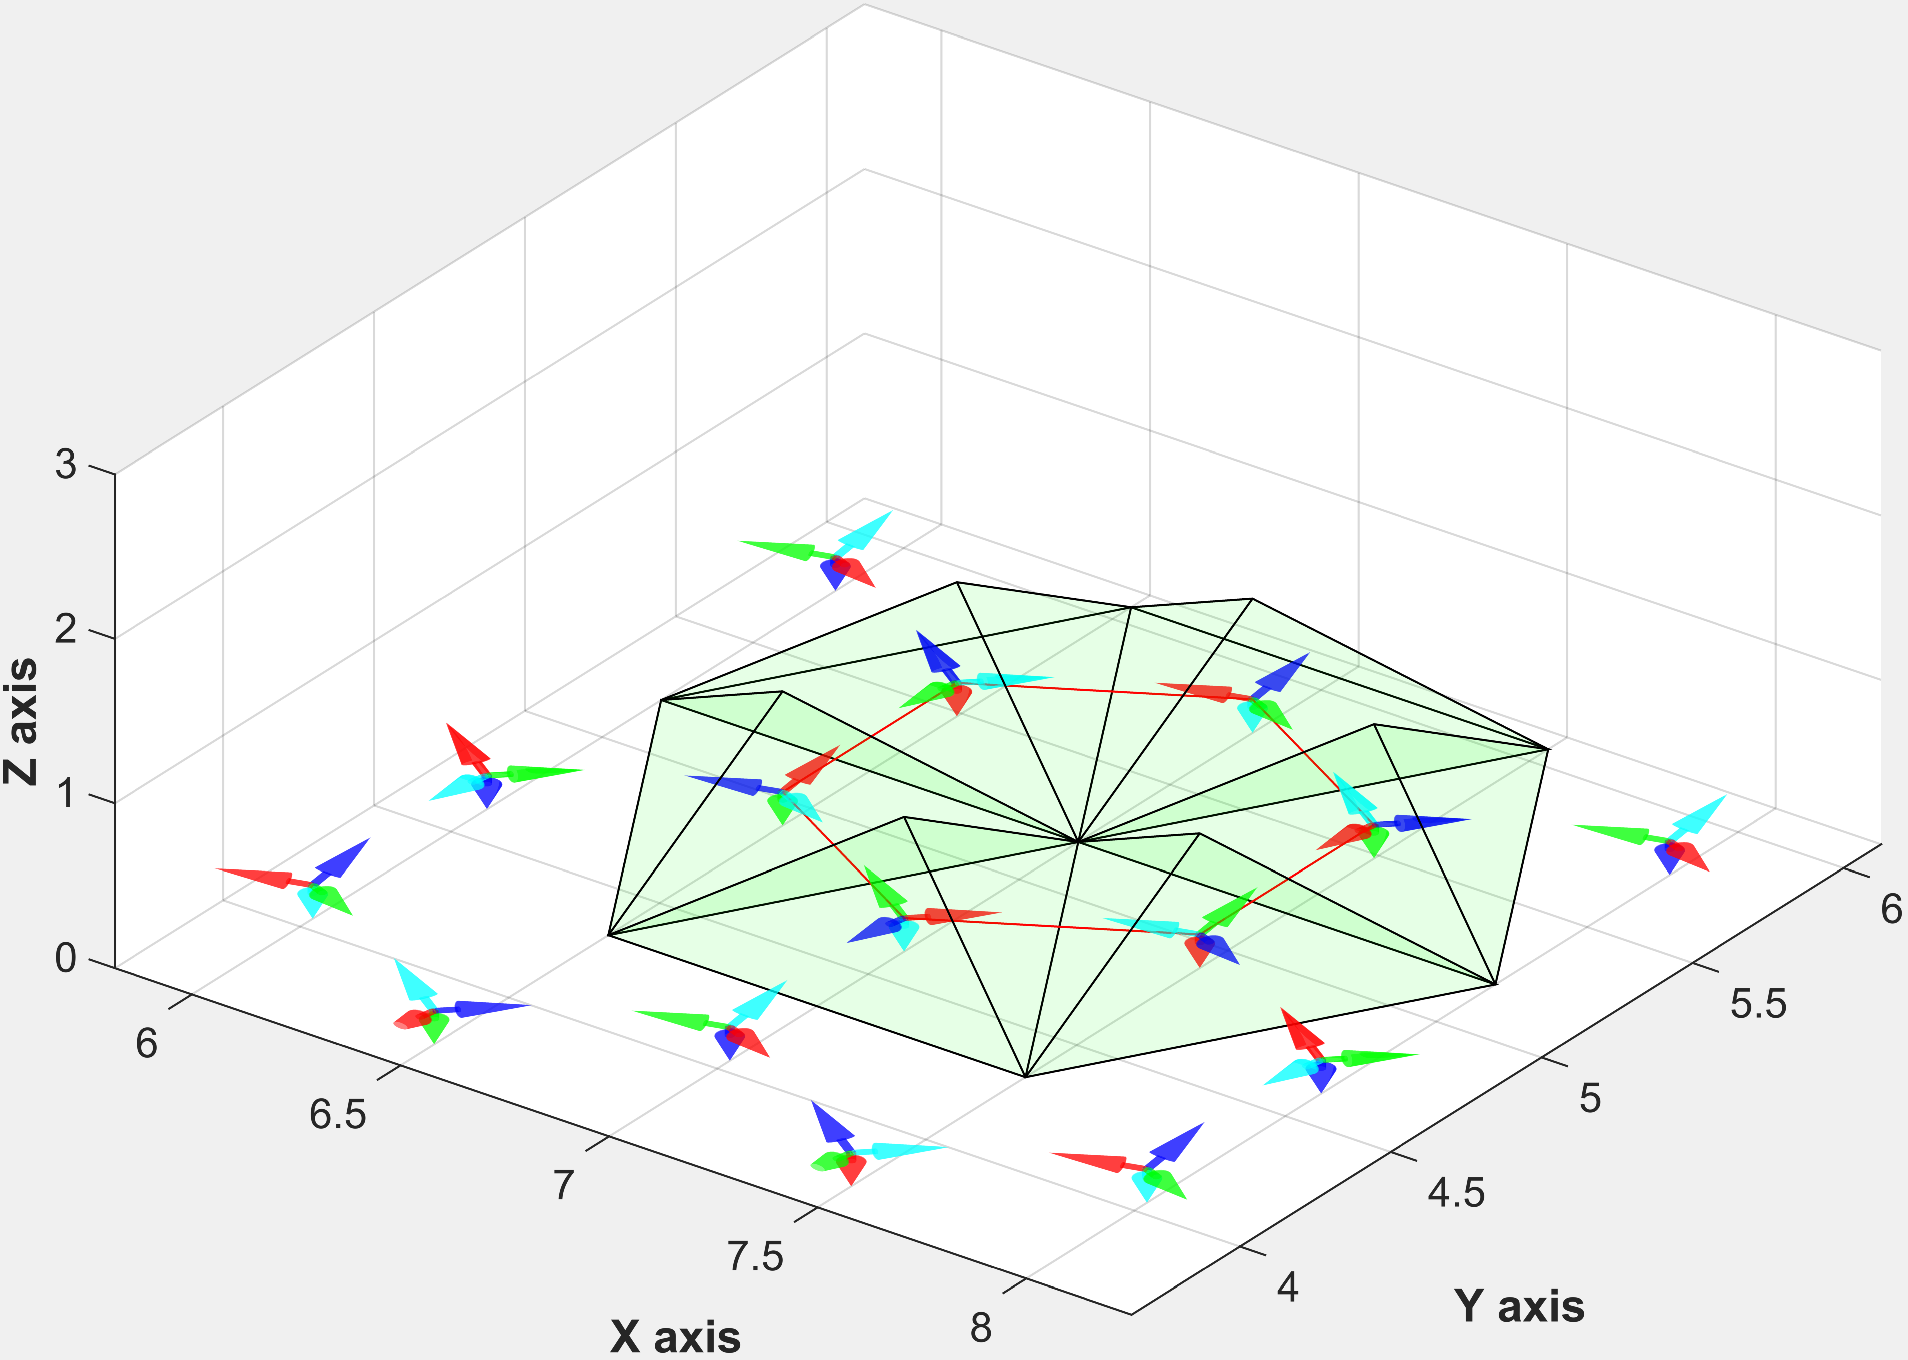
\includegraphics[width=0.5\textwidth]{image/tetraPath1.pdf}
	\label{fig:Tetra2Case1}
	}
\caption{Blah Blah Tetra}
\end{figure}
\end{center}
%%
%%
%%
%%==================================================================================
%%
%%==================================================================================
%%
%%
%%
\clearpage
\newpage
\noindent\uline{\textbf{Octahedron solid}}:
Dennis also went his own way and divided the sides of the triangles into equal-angles (as measured from the center of the geodesic), instead of equal-length pieces. This technique is slightly more effective at evenly distributing the triangles across the surface of the sphere. For example, compare an octahedron subdivided with frequency 20, using the linear technique (as outlined by the quiz) versus the angular technique Dennis used in this picture. Note how the linear technique has the triangles piling up along the edges of the original face of the octahedron, where the radial technique does a better job of spacing them out.\\

\begin{center}
\begin{figure}[h]
\subfigure[The first shortest path of Octahedron path rolling]{
	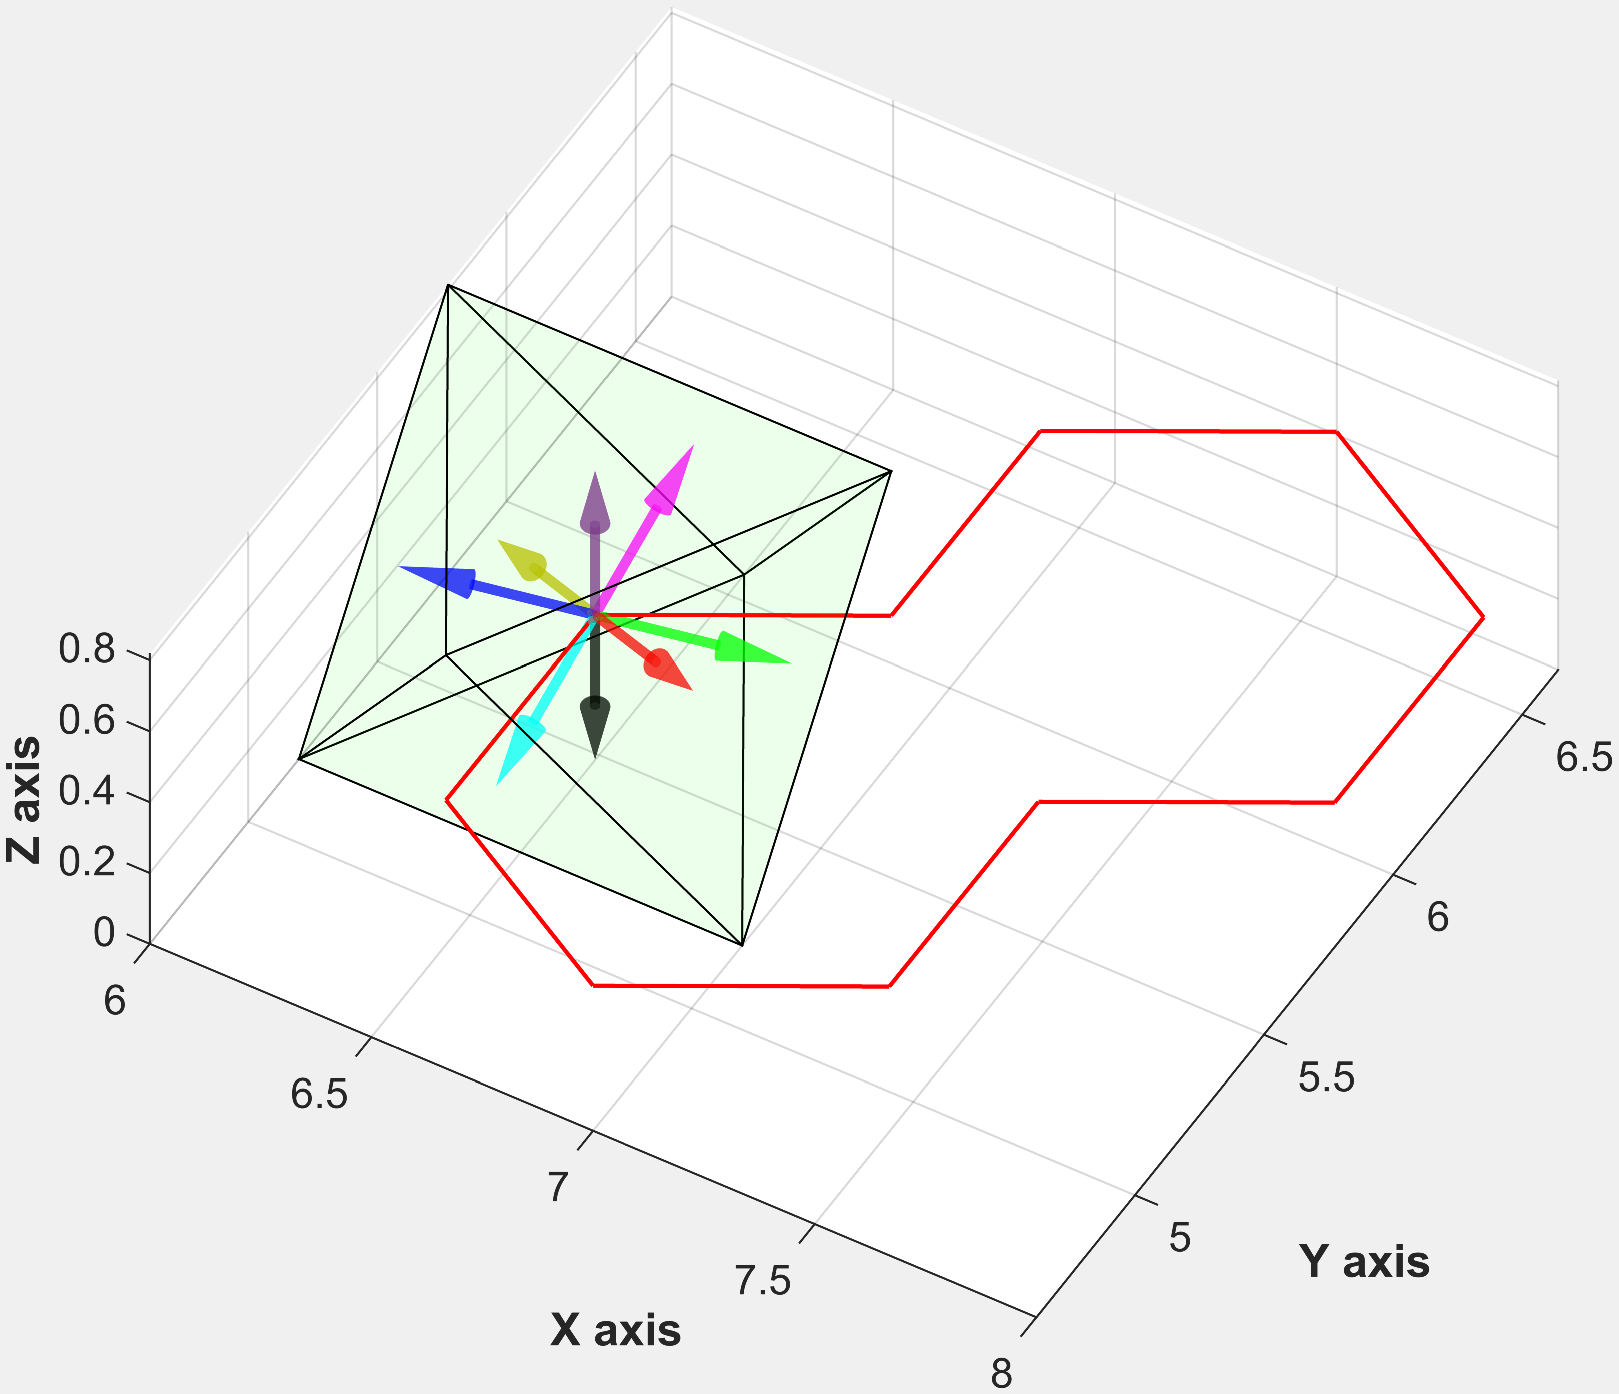
\includegraphics[width=0.5\textwidth]{image/octoPath1.pdf}
	\label{fig:Octa1Case1}
	}
\hfill
\subfigure[The second shortest path of Octahedron path rolling]{
	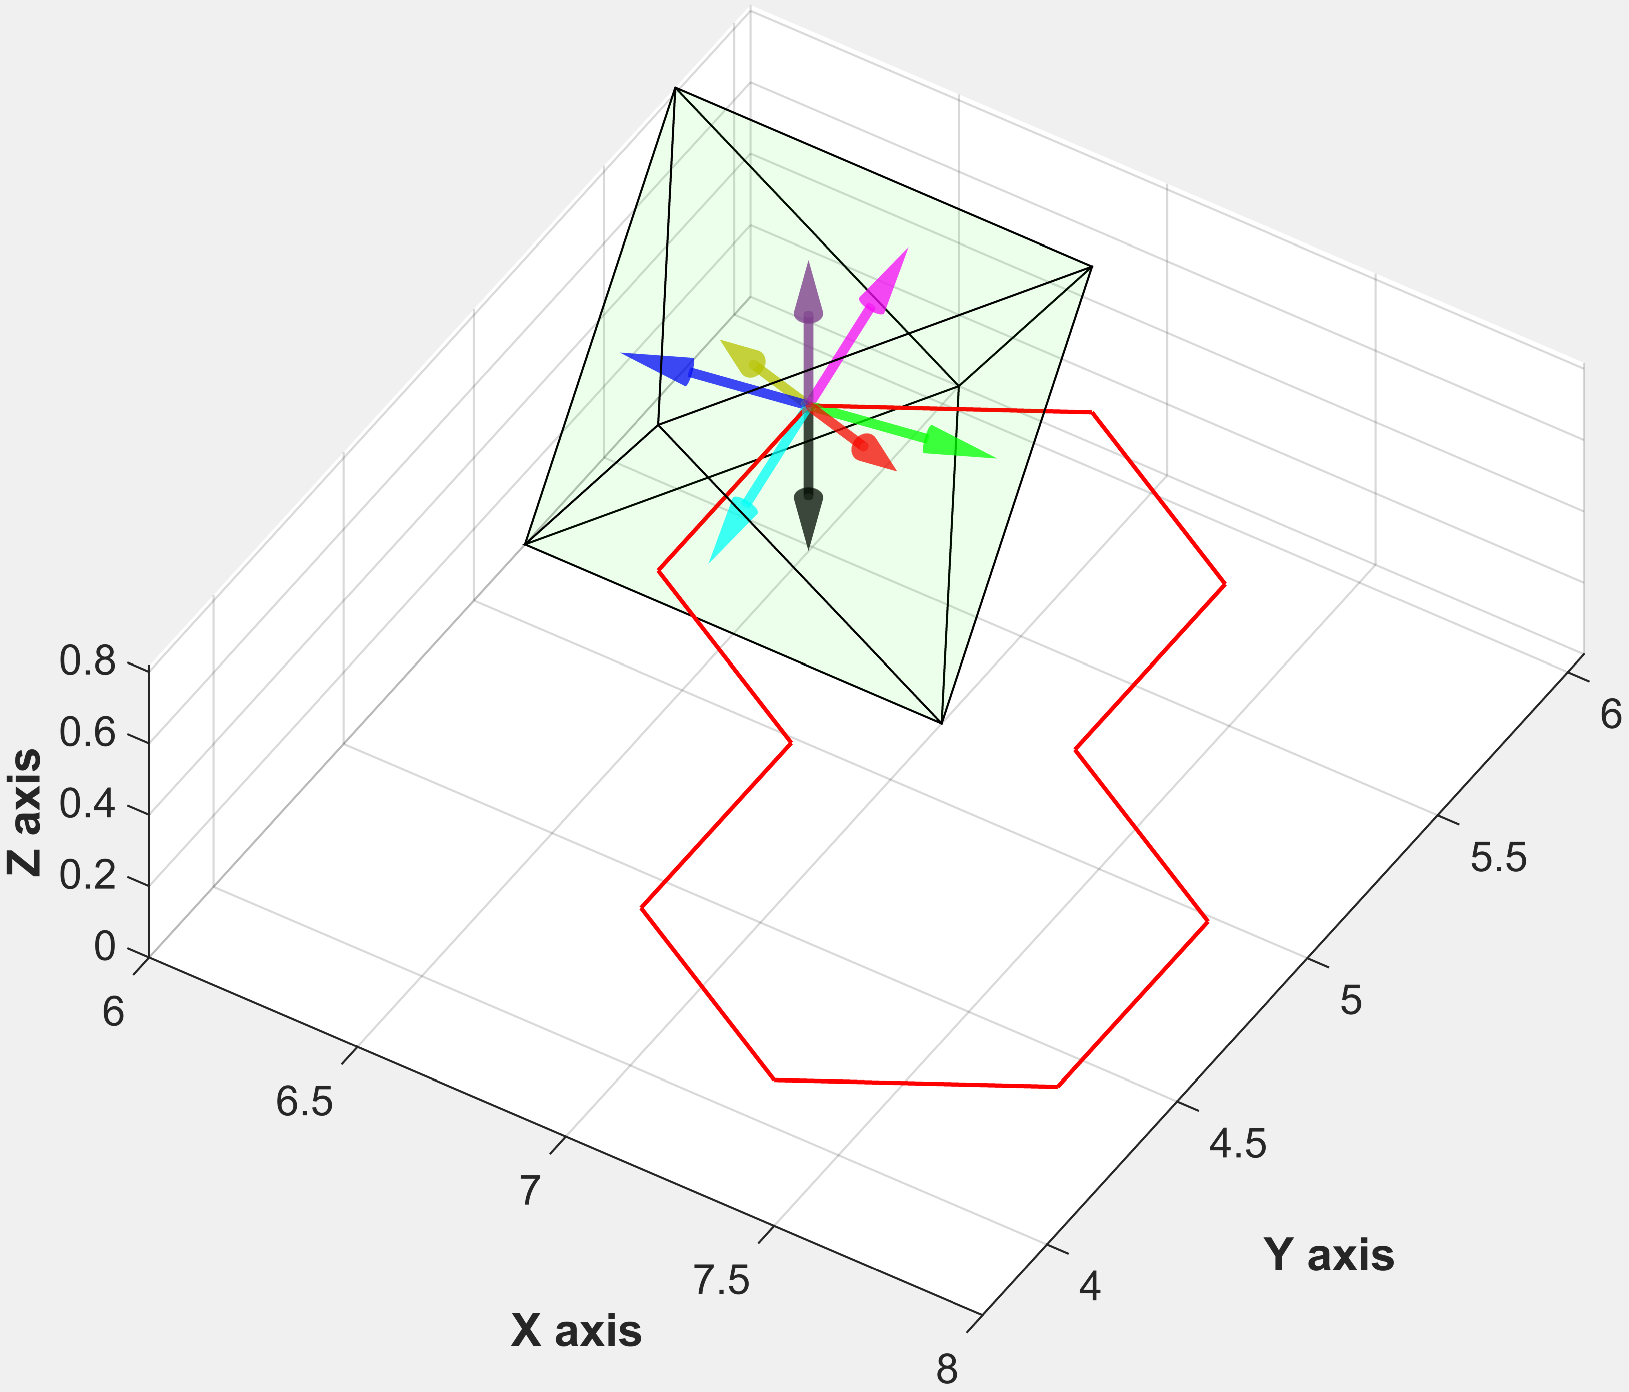
\includegraphics[width=0.5\textwidth]{image/octoPath2.pdf}
	\label{fig:Octa1Case1}
	}
\caption{Blah Blah Octa}
\end{figure}
\end{center}
%%
%%
%%
%%==================================================================================
%%
%%==================================================================================
%%
%%
%%
\clearpage
\newpage
\noindent\uline{\textbf{Icosahedron solid}}:
Writing about cube solid properties\\
This is the rolling path of icosahedron type \ref{fig:icosaPaths}.
\begin{center}
\begin{figure}[h]
\subfigure[The first shortest path of Icosahedron path rolling]{
	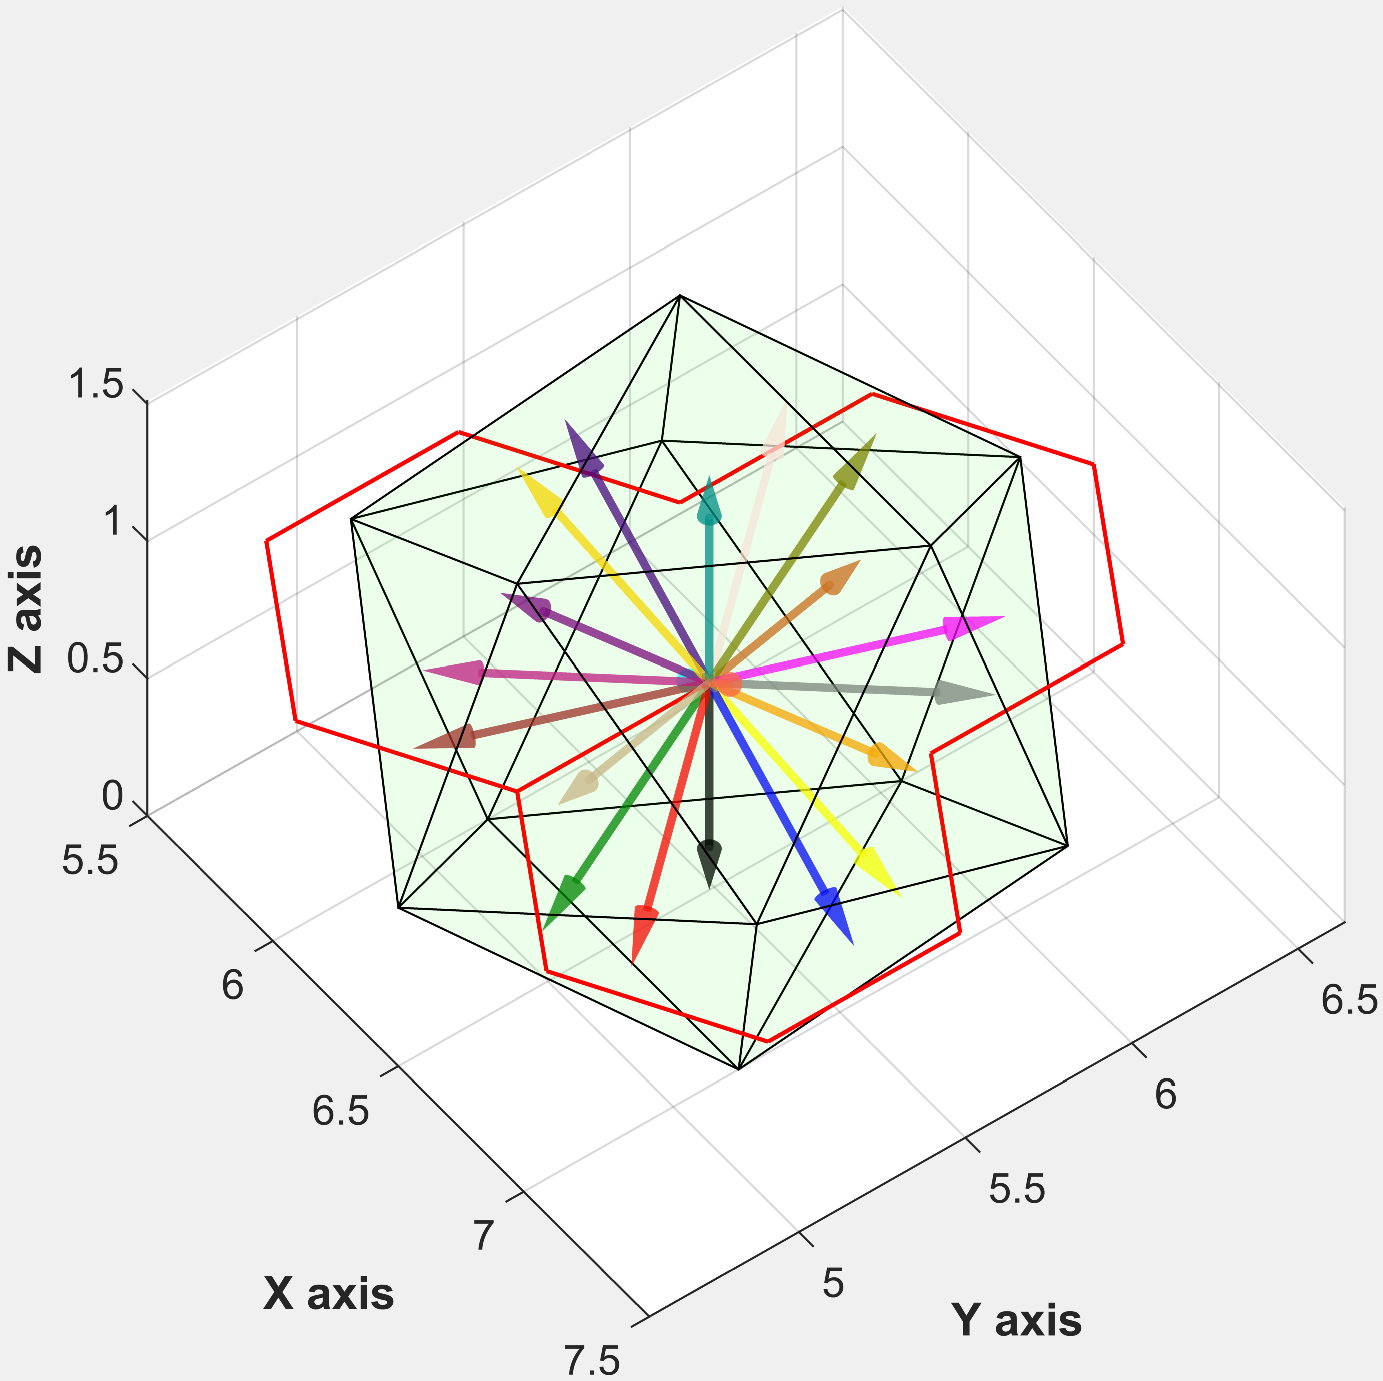
\includegraphics[width=0.5\textwidth]{image/icosaPath.pdf}
	\label{fig:Octa1Case1}
	}
\hfill
\subfigure[The top view of path planning for Icosahedron]{
	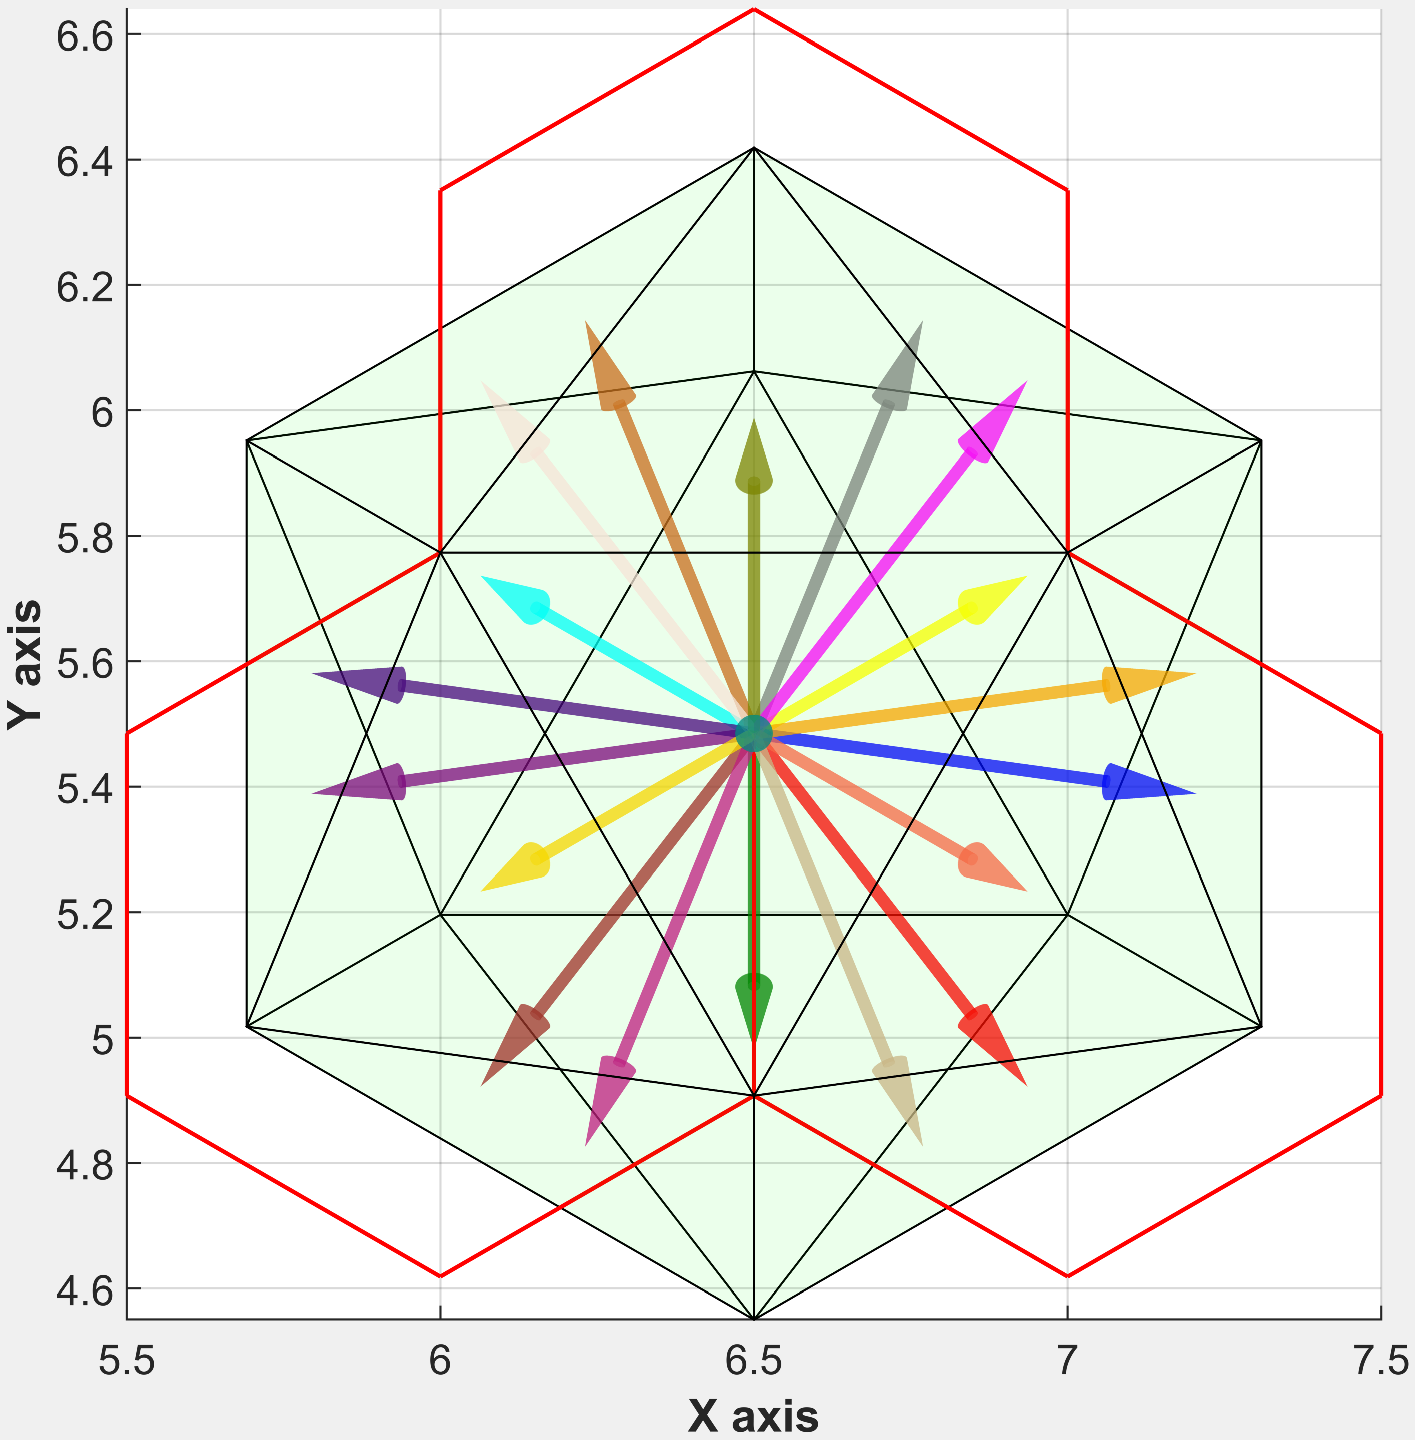
\includegraphics[width=0.5\textwidth]{image/icosaPathTopView.pdf}
	\label{fig:Octa1Case1}
	}
\caption{Blah Blah Octa}
\label{fig:icosaPaths}
\end{figure}
\end{center}
%
\clearpage
\newpage
\noindent\uline{\textbf{Dodecahedron}}:

%\noindent\uline{Result}: 
%\begin{figure}[h]
%\centering
%	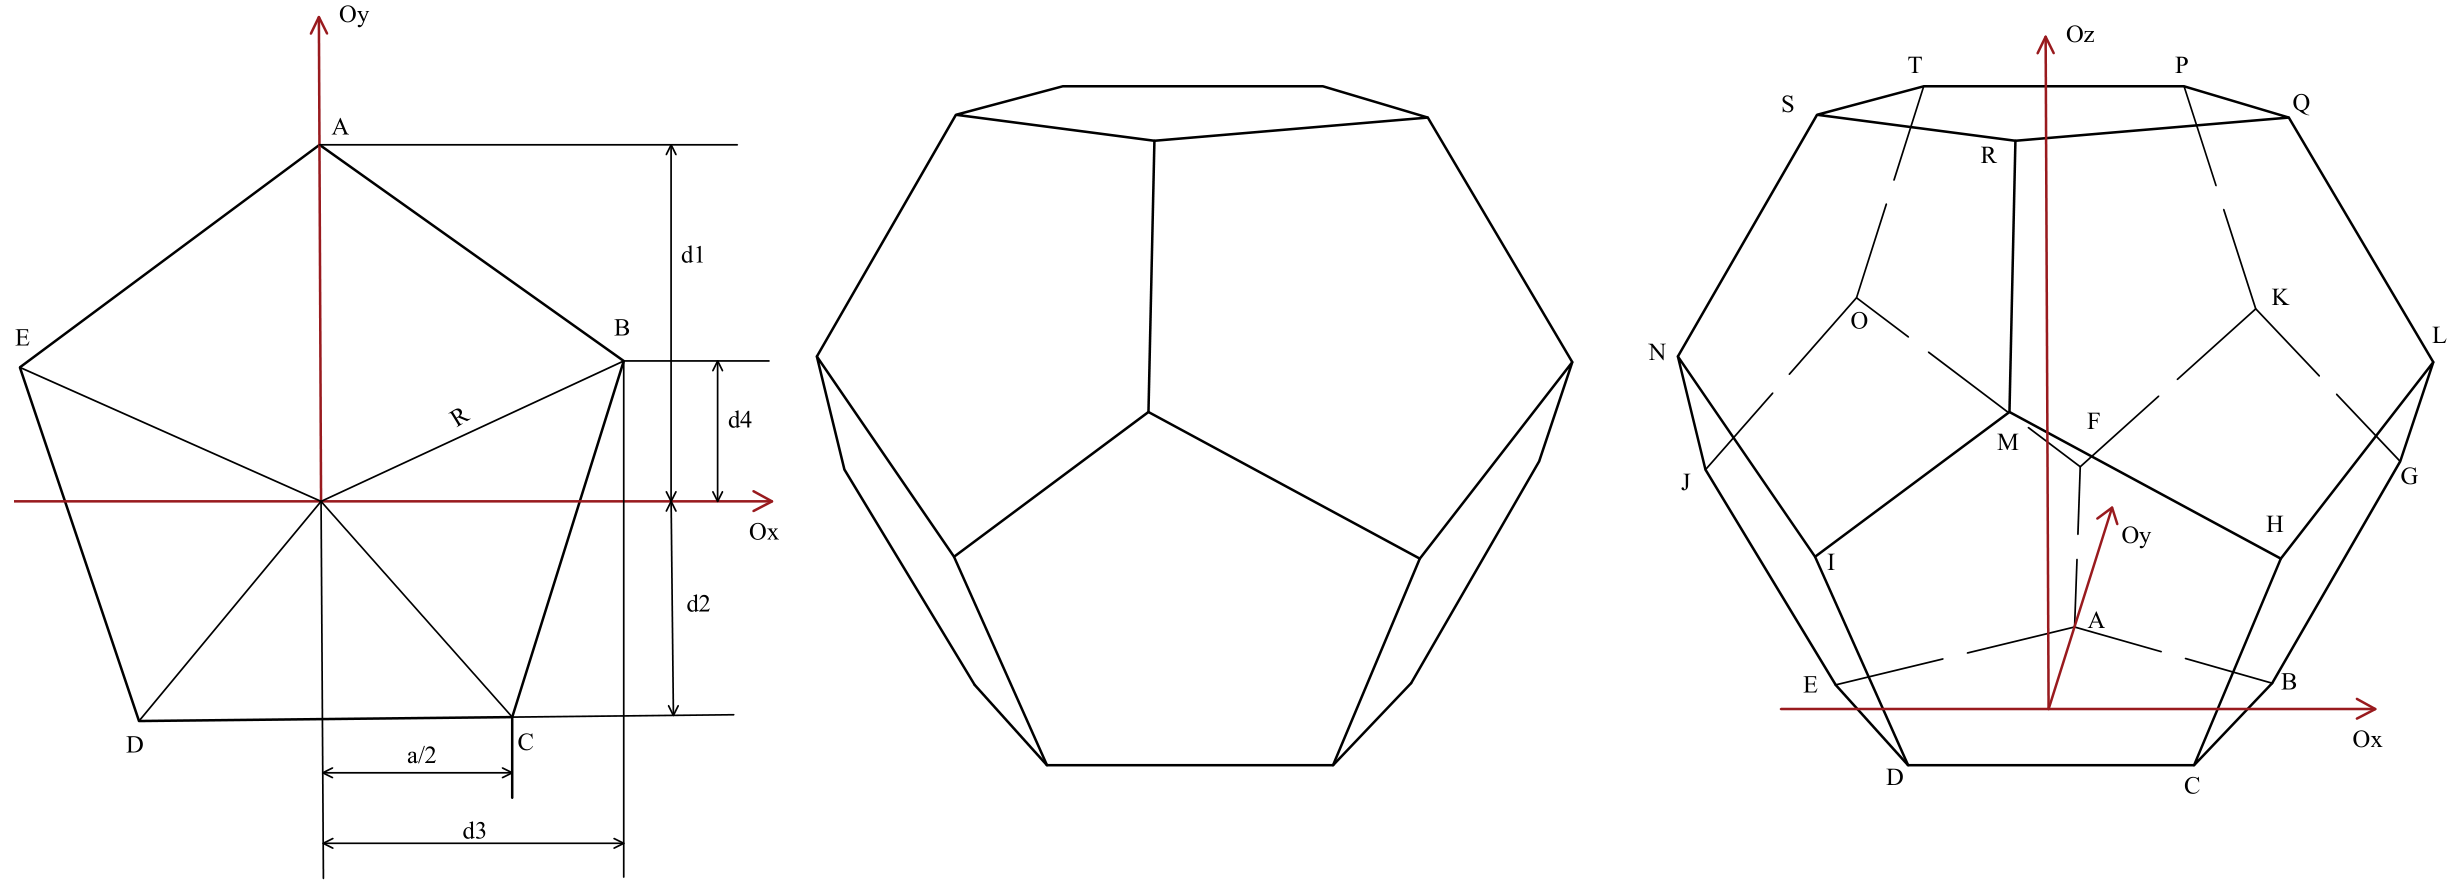
\includegraphics[width=1\textwidth]{image/dodecahedron1.png}
%	\caption{Shortest path of cube rolling}
%	\label{fig:dodecahedron1}
%\end{figure}

\noindent\uline{Properties}: 
An dodecahedron has 12 faces and 20 vertices of which generates a pentagon as shown in Figure \ref{fig:dodecahedron2}.
It will be assumed that the coordinates $Oxyz$ lie on $ABCDE$ surface within $Oy$ through $A$ and $Oz$ perpendicular to $ABCDE$.
The 30 edges have the same length as $a$. It should be determined all the vertices' coordinates in the three dimensional system.
The Figure \ref{fig:dodecahedron2} indicates the lengths of each vertices from $l_1$ to $l_4$ and the angles $\alpha_1$ to $\alpha_4$ which correspond to the five sides of a pentagon.

\begin{figure}[h]
\centering
	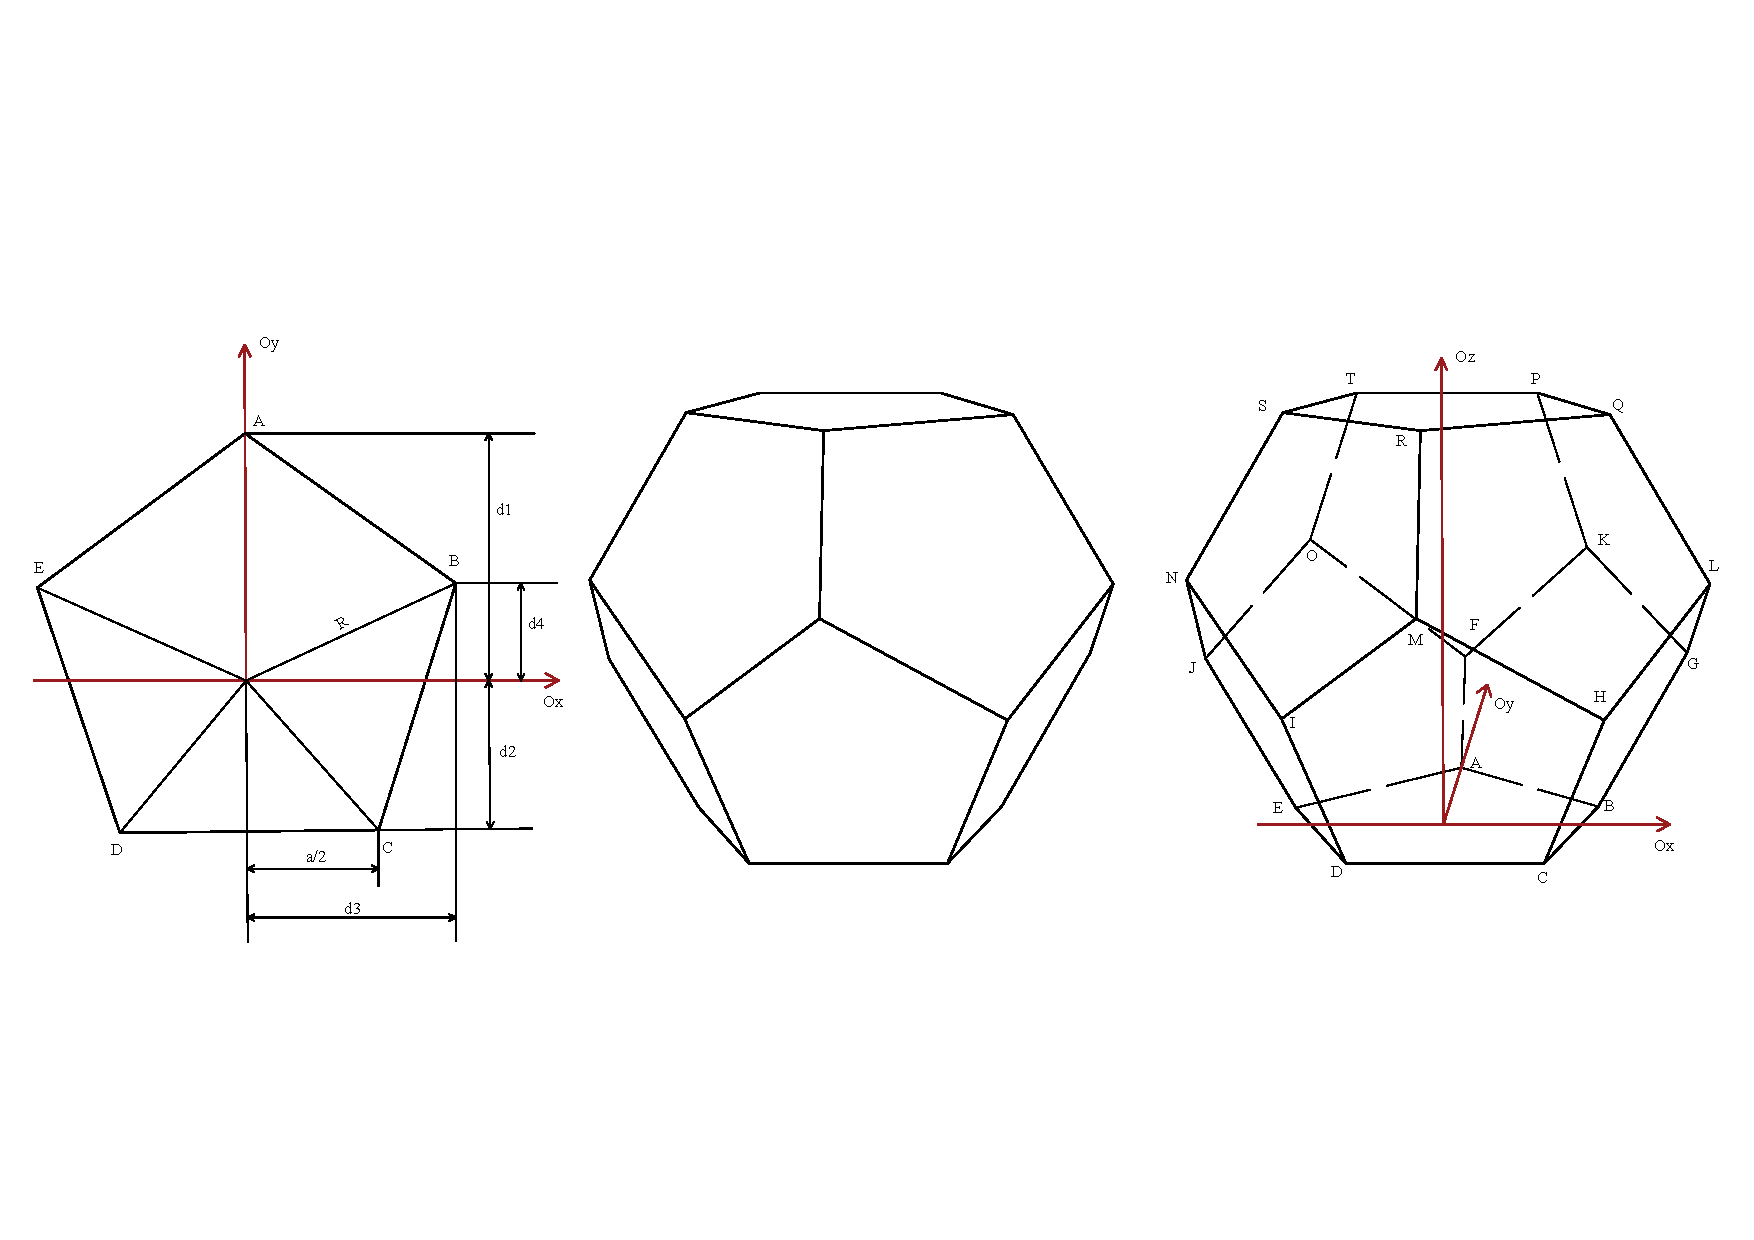
\includegraphics[width=1\textwidth]{image/dodecahedron2.pdf}
	\caption{Dodecahedron's vertices.}
	\label{fig:dodecahedron2}
\end{figure}

The path planning will implement on a surface but it will be considered in $3D$ spaces. Then, each of vertices will be determined on $3D$ coordinates such as the vertices $A$ has coordinate with $[A_x A_y A_z]$. Based on the properties of pentagon, the angle $\alpha_1=\frac{2\pi}{5}$ and $\alpha_4=\frac{\pi}{5}$. Because the angle between $Ox$ and $Oy$ is $\frac{\pi}{2}$, the sum of $\alpha_1$ and $\alpha_2$ is $\alpha_1 + \alpha_2 = \frac{\pi}{2}$. Then the other two angles $\alpha_2$ and $\alpha_3$ can be determined by $\alpha_2 = \frac{\pi}{2}-\alpha_1 = \frac{\pi}{2}-\frac{2\pi}{5} = \frac{\pi}{10}$ and $\alpha_3 = \alpha_1-\alpha_2 = \frac{2\pi}{5}-\frac{pi}{10} = \frac{3\pi}{10}$.\\

From the Figure \ref{fig:dodecahedron2}(c), these labelled dimensions can be calculated as $l_1 = R_d = \frac{a}{2\sin{\alpha_4}}$ with $R_d$ is the circumradius of dodecahedron, $l_2 = l_1\cos{\alpha_4}$, $l_3 = l_1\cos{\alpha_2}$, and $l_4 = l_1\sin{\alpha_2}$. Referencing to the properties of a dodecahedron with length $a$, the radius of an inscribed sphere is $r_i = \frac{a}{20}\sqrt{10(25+11\sqrt{5})}$ and the circumscribed sphere radius is $r = a\frac{\sqrt{3}}{2}\frac{1+\sqrt{5}}{2}$.\\

There are total $20$ vertices of a dodecahedron. This article focuses on the rolling contact to $2D$ surface, the bottom surface of the dodecahedron integrated to the $Oxy$ which contact to the $2D$ surface. This condition express the $Oz$ dimension of the vertices $ABCDE$ equal to $0$ or $A_z = B_z = C_z = D_z = E_z = 0$. Then $P_z = Q_z = R_z = S_z = T_z = 2.r_i = \frac{a}{10}\sqrt{10(25+11\sqrt{5})}$.\\

It can be seen that the distance $|AF|$ is $a$ and the distance $|BF|$ is $2l_3$. Using the distance properties and squaring the results give:
\begin{equation} 
\label{dodeca:eq1}
\begin{split}
AF^2 & = a^2 = (A_x-F_x)^2 + (A_y-F_y)^2 + (A_z-F_z)^2 \\
BF^2 & = (2l_3)^2 = (B_x-F_x)^2 + (B_y-F_y)^2 + (B_z-F_z)^2
\end{split}
\end{equation}

Figure \ref{fig:dodecahedron2}(d) shows that $A_x = F_x = 0$, $A_y = l_1$, $B_y = l_4$, $B_x = l_3$, $A_z = B_z$. Define $l_5=A_z-F_z$, the relations of these equations are:
\begin{equation} 
\label{dodeca:eq2}
\begin{split}
a^2 & = (F_y-l_1)^2 + l_5^2\\
(2l_3)^2 & = (F_y-l_4)^2 + l_5^2 + l_3^2
\end{split}
\end{equation}

Solving $F_y$ and $l_5$ gives:
\begin{equation} 
\label{dodeca:eq3}
\begin{split}
F_y & = \frac{a^2-(2l_3)^2-(l_1^2-l_3^2-l_4^2)}{2(l_4-l_1)} \\
l_5 & = \frac{1}{\sqrt{2}}\sqrt{a^2+(2l_3)^2-(F_y-l_1)^2-(F_y-l_4)^2-l_3^2}
\end{split}
\end{equation}

From these equations \ref{dodeca:eq1},\ref{dodeca:eq2},\ref{dodeca:eq3}, all the vertices will be founded in the three-dimensional space. Path planning based on rolling is the motion of all these vertices through edges' contact.


%%
%%
%%
%%==================================================================================
%
%\begin{figure}[h]
%\centering
%	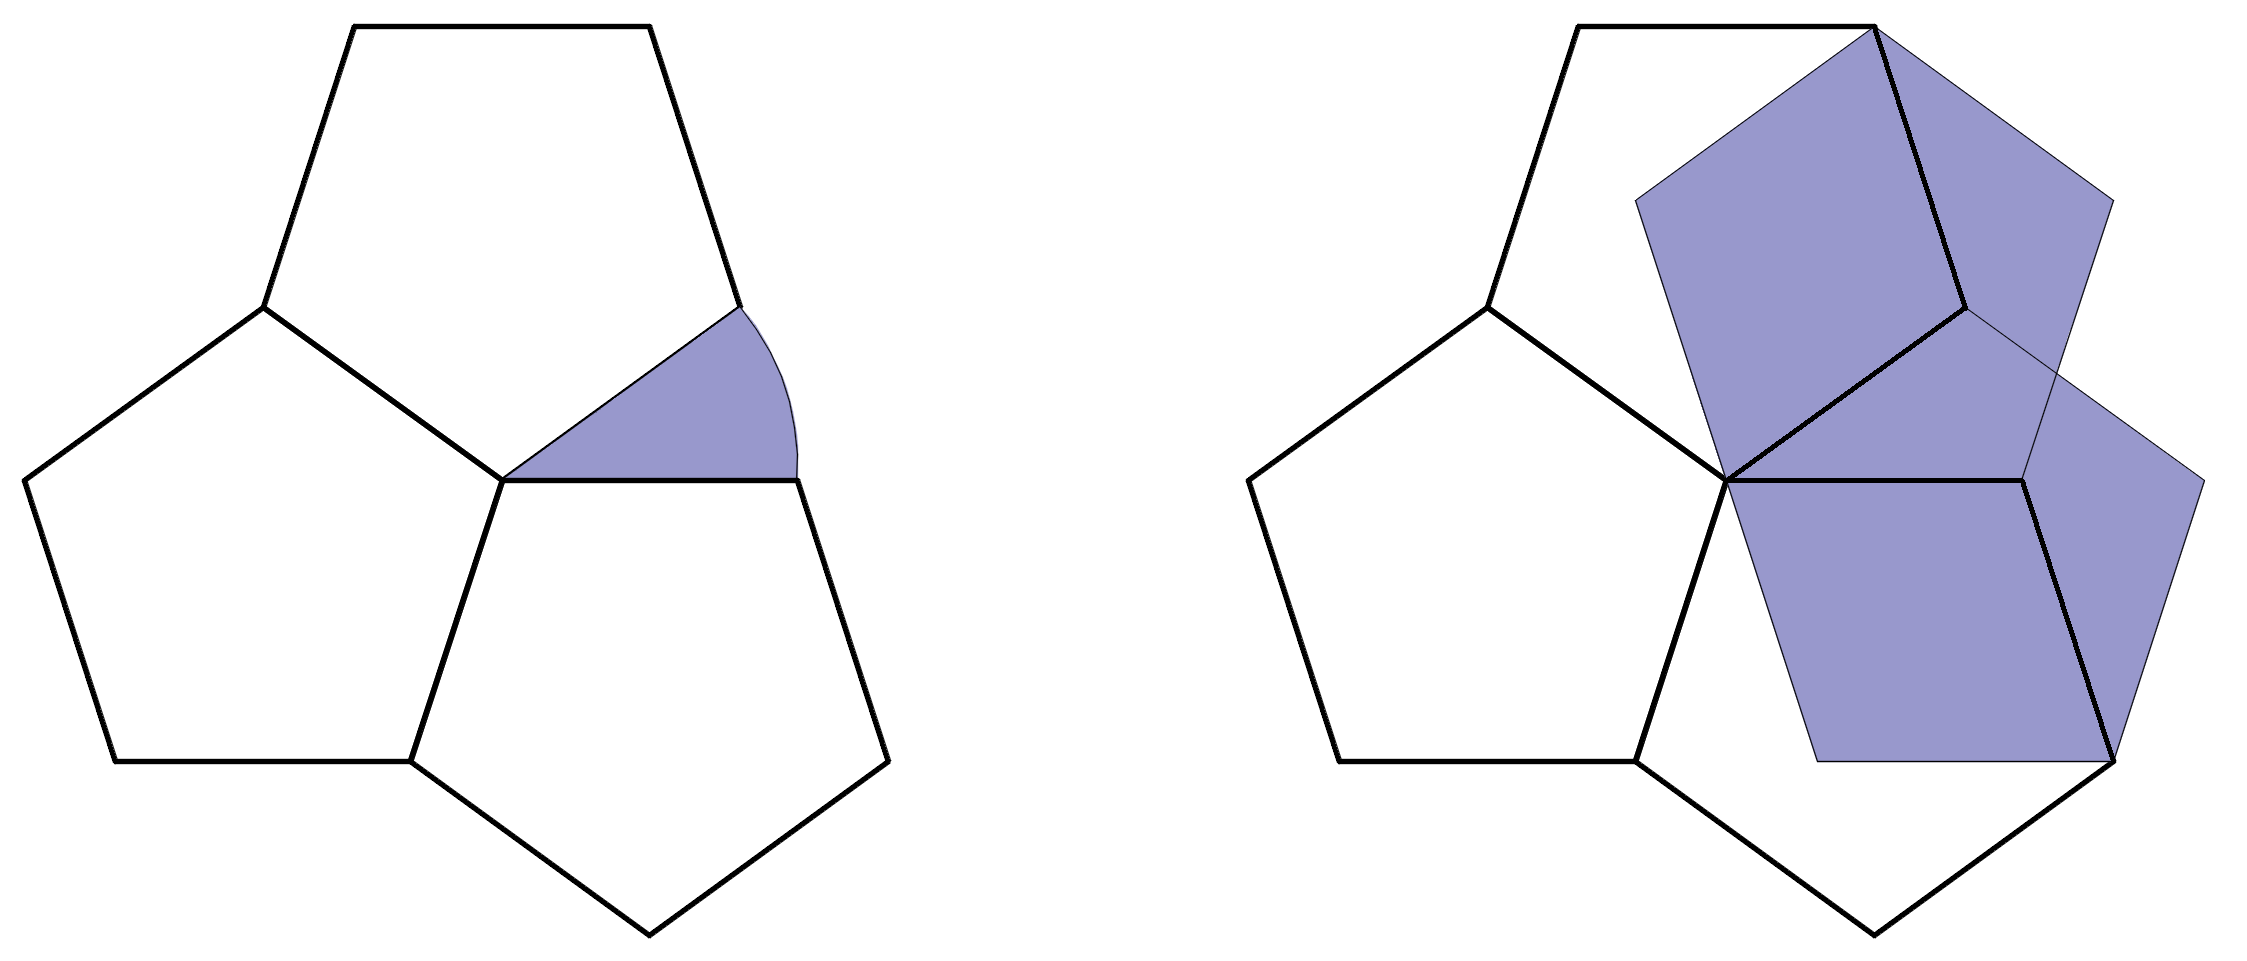
\includegraphics[width=1\textwidth]{image/dodecaOverlap.png}
%	\caption{Pentagons connect around a point with a gap and overlap}
%	\label{fig:dodecaOverlap}
%\end{figure}
%%==================================================================================
%%
%%
%%
\newpage
\noindent\uline{\textbf{Experiments}}:
Writing about cube solid properties\\

\noindent\uline{\textbf{Discussion}}: 
\textcolor{blue}{Q2 \& Q3\\
- Q2: What are the new things you learned after you did whatever you did?\\
- Q3: What exactly did you do?}\\

\begin{itemize}
\color{red}
\item \textbf{Discussion}
\item \textit{What your results mean}
\item \textit{Why it makes a difference}
\item \textbf{Conclusion}
\item \textit{Broader implications}
\item \textit{Areas for further study}
\end{itemize}





